% CS301 Week 1 -- where your data lives: structured programming, pointers,
% dynamic memory, and ADTs
% Difficulty: intro (rebuilt 2026-08-13 per instructor's course-wide default
% change in .claude/rules/knowledge-base-CS301.md). Motivation-heavy; a worked
% example sits within 1 slide of every definition; one new symbol per frame;
% more, shorter frames than the prior core-tier deck. Proofs/derivations are
% not applicable to this lecture's content, so the "proofs omitted" intro-tier
% clause has no bite here -- everything below is definition + trace, matching
% intro's "results stated with intuition" spirit.
% Page-grounded in Wirth2004 p.111, Sedgewick2011 pp.64/120, Karumanchi2017
% p.18 (PDF); Horowitz & Sahni and Aho-Hopcroft-Ullman cited at chapter level
% only (not yet page-indexed -- see knowledge-base-CS301.md Anchor Textbooks).

\documentclass[aspectratio=169]{beamer}
% =============================================================================
% Preambles/header.tex — shared LaTeX/Beamer preamble for this project
%
% Use from a Beamer lecture by prepending:
%     % =============================================================================
% Preambles/header.tex — shared LaTeX/Beamer preamble for this project
%
% Use from a Beamer lecture by prepending:
%     % =============================================================================
% Preambles/header.tex — shared LaTeX/Beamer preamble for this project
%
% Use from a Beamer lecture by prepending:
%     \input{header}
% and compiling with TEXINPUTS=../Preambles:$TEXINPUTS (the /compile-latex
% skill does this automatically).
%
% PALETTE CONTRACT. Color names defined here MUST match the names in
% Quarto/theme-template.scss so Beamer and Quarto renderings use the same
% palette. The scripts/check-palette-sync.sh script enforces this.
%
% To customize: edit the HEX values below AND the matching $variable in
% Quarto/theme-template.scss, then run scripts/check-palette-sync.sh.
%
% TITLE PAGE. A formal, serif (Libertine) title-page template is defined in
% the Beamer-only block below (\setbeamertemplate{title page}) -- title,
% subtitle, a thin gold rule, then \author/\institute/\date. Frametitle and
% body text remain on Beamer's sans-serif default. No SCSS counterpart is
% needed for this (font/layout only, no new colors).
% =============================================================================

% -----------------------------------------------------------------------------
% Engine detection + encoding
%
% Our /compile-latex skill uses XeLaTeX, where inputenc is unnecessary and
% can produce encoding warnings. Only load inputenc under pdfTeX.
% -----------------------------------------------------------------------------
\usepackage{iftex}
\ifPDFTeX
  \usepackage[utf8]{inputenc}
\fi

\usepackage{amsmath, amssymb, amsthm}
\usepackage{booktabs}
\usepackage{graphicx}

% -----------------------------------------------------------------------------
% Serif face for the title page (formal/academic look). Linux Libertine is
% XeLaTeX- and pdfTeX-safe and redefines \rmdefault, so \rmfamily picks it up
% everywhere \rmfamily is used explicitly. Body text and frametitles stay on
% Beamer's own sans-serif default (unaffected) -- only the title-page
% \setbeamerfont{...} overrides below opt in to \rmfamily.
% -----------------------------------------------------------------------------
\usepackage{libertine}

% -----------------------------------------------------------------------------
% PALETTE — mirrors Quarto/theme-template.scss variable names.
% Load xcolor and define colors BEFORE anything that references them
% (notably hyperref, hypersetup, and the Beamer color assignments).
% -----------------------------------------------------------------------------
\usepackage{xcolor}

\definecolor{primary-blue}{HTML}{012169}      % headings, accents
\definecolor{primary-gold}{HTML}{B9975B}      % emphasis, borders
\definecolor{highlight-yellow}{HTML}{F2A900}  % markers, alerts
\definecolor{light-bg}{HTML}{E8EDF5}          % title / section backgrounds
\definecolor{jet}{HTML}{1A1A1A}               % body text

% Semantic colors (used in diagrams and annotations)
\definecolor{positive}{HTML}{15803D}          % good / observed / identified
\definecolor{negative}{HTML}{B91C1C}          % bad / problematic / bias
\definecolor{neutral}{HTML}{525252}           % reference / context

% Highlight accents (match .hi-* classes in the SCSS)
\definecolor{hi-slate}{HTML}{314F4F}
\definecolor{hi-green}{HTML}{2E8B57}
\definecolor{hi-red}{HTML}{C41E3A}

% Semantic aliases so skill templates and snippets can write
% \textcolor{accent}{...} without hard-coding "primary-blue".
\colorlet{accent}{primary-blue}
\colorlet{accent2}{primary-gold}

% -----------------------------------------------------------------------------
% Hyperref — loaded AFTER xcolor + palette so link colors resolve.
% -----------------------------------------------------------------------------
\usepackage{hyperref}
\hypersetup{colorlinks=true, linkcolor=primary-blue, urlcolor=primary-blue,
            citecolor=primary-blue, pdfborder={0 0 0}}

% -----------------------------------------------------------------------------
% Course code — set once per deck (after \input{header}, before \begin{document})
% via \coursecode{CS401}. Shown in the footer on every slide so a deck's course
% is identifiable without opening the title page. Empty by default.
% -----------------------------------------------------------------------------
\makeatletter
\newcommand{\coursecode}[1]{\gdef\@coursecodetext{#1}}
\gdef\@coursecodetext{}
\makeatother

% -----------------------------------------------------------------------------
% Beamer theme assignments (only apply under Beamer).
%
% We detect Beamer via \@ifclassloaded{beamer}, which is the documented,
% non-internal way. This must be wrapped in \makeatletter/\makeatother
% because \@ifclassloaded contains an @-catcode character.
% -----------------------------------------------------------------------------
\makeatletter
\@ifclassloaded{beamer}{%
  \usefonttheme{professionalfonts}
  \setbeamercolor{structure}{fg=primary-blue}
  \setbeamercolor{frametitle}{fg=primary-blue}
  \setbeamercolor{title}{fg=primary-blue}
  \setbeamercolor{subtitle}{fg=primary-gold}
  \setbeamercolor{author}{fg=primary-blue}
  \setbeamercolor{institute}{fg=neutral}
  \setbeamercolor{date}{fg=primary-gold}
  \setbeamercolor{itemize item}{fg=primary-blue}
  \setbeamercolor{itemize subitem}{fg=primary-gold}
  \setbeamercolor{alerted text}{fg=primary-gold}
  \setbeamercolor{block title}{fg=white, bg=primary-blue}
  \setbeamercolor{block body}{bg=light-bg}
  % Semantic block variants: block=definition/concept (blue), exampleblock=
  % worked example (green/positive), alertblock=key takeaway or caution (gold).
  % Keep to <=2 colored boxes per slide across ALL three variants (INV-7).
  \setbeamercolor{block title example}{fg=white, bg=positive}
  \setbeamercolor{block body example}{bg=light-bg}
  \setbeamercolor{block title alerted}{fg=white, bg=primary-gold}
  \setbeamercolor{block body alerted}{bg=light-bg}

  % ---------------------------------------------------------------------------
  % Formal title page: serif (Libertine, via \rmfamily) for title-page
  % elements only. Body text, itemize, and frametitle are intentionally left
  % on Beamer's sans-serif default -- \usebeamerfont{title} is also what
  % \transitionslide (below) uses for its big centered text, so section
  % transitions pick up the same serif treatment for free.
  % ---------------------------------------------------------------------------
  \setbeamerfont{title}{family=\rmfamily, series=\bfseries, size=\Large}
  \setbeamerfont{subtitle}{family=\rmfamily, shape=\itshape, size=\normalsize}
  \setbeamerfont{author}{family=\rmfamily, size=\normalsize}
  \setbeamerfont{institute}{family=\rmfamily, size=\scriptsize}
  \setbeamerfont{date}{family=\rmfamily, size=\scriptsize}

  \setbeamertemplate{title page}{
    \vfill
    \begin{center}
      {\usebeamerfont{title}\usebeamercolor[fg]{title}\inserttitle\par}
      \vspace{0.15cm}
      {\usebeamerfont{subtitle}\usebeamercolor[fg]{subtitle}\insertsubtitle\par}
      \vspace{0.45cm}
      {\color{primary-gold}\rule{0.42\textwidth}{0.6pt}\par}
      \vspace{0.45cm}
      {\usebeamerfont{author}\usebeamercolor[fg]{author}\insertauthor\par}
      \vspace{0.35cm}
      {\usebeamerfont{institute}\usebeamercolor[fg]{institute}\insertinstitute\par}
      \vspace{0.35cm}
      {\usebeamerfont{date}\usebeamercolor[fg]{date}\insertdate\par}
    \end{center}
    \vfill
  }

  % Minimal footer: course code (left) + page X / N (right), no navigation clutter
  \setbeamertemplate{navigation symbols}{}
  \setbeamertemplate{footline}{%
    \color{neutral}\footnotesize\hspace{0.7em}\@coursecodetext\hfill
    \insertframenumber/\inserttotalframenumber\hspace{0.7em}\vspace{0.3em}}
}{}
\makeatother

% -----------------------------------------------------------------------------
% TikZ setup — libraries the snippet gallery uses
% -----------------------------------------------------------------------------
\usepackage{tikz}
\usetikzlibrary{arrows.meta, positioning, calc, decorations.pathreplacing,
                fit, shapes.geometric, backgrounds}

% Shared TikZ styles — snippets and hand-written diagrams can pick these up
% via `\begin{tikzpicture}[every node/.style={...}]` or by naming specific
% styles (e.g., `\node[dag-node] (X) at (0,0) {X};`).
\tikzset{
  % Node styles for causal DAGs and similar
  dag-node/.style = {
    draw=primary-blue, fill=light-bg, rounded corners=2pt,
    minimum width=1.2cm, minimum height=0.9cm, align=center, font=\small
  },
  decision-node/.style = {
    draw=primary-gold, fill=white, diamond, aspect=1.8,
    minimum width=1.8cm, minimum height=1.2cm, align=center, font=\small,
    inner sep=1pt
  },
  % Edge styles — observed vs counterfactual
  observed-edge/.style = {-{Latex[length=2.5mm]}, thick, draw=jet},
  counterfactual-edge/.style = {-{Latex[length=2.5mm]}, thick, draw=neutral, dashed},
  confound-edge/.style = {-{Latex[length=2.5mm]}, thick, draw=negative, dashed},
  % Data-point styles for plots
  observed-dot/.style = {fill=primary-blue, draw=primary-blue, circle, inner sep=1.2pt},
  counterfactual-dot/.style = {fill=white, draw=neutral, circle, inner sep=1.2pt}
}

% -----------------------------------------------------------------------------
% Convenience macros
% -----------------------------------------------------------------------------
\newcommand{\muted}[1]{\textcolor{neutral}{#1}}
\newcommand{\key}[1]{\textcolor{primary-gold}{\textbf{#1}}}
\newcommand{\good}[1]{\textcolor{positive}{#1}}
\newcommand{\bad}[1]{\textcolor{negative}{#1}}

% Standout frame macro: full-bleed dark background for section transitions.
% Beamer-only (uses \begin{frame}/\setbeamercolor/\usebeamerfont) -- do not
% call from an article-class file (e.g. Notes/<CODE>/*-notes.tex). \muted,
% \key, \good, \bad, and \coursecode above are plain xcolor/gdef and are
% safe to use from either class; verified when Notes/article-class support
% was added.
% Expand: \transitionslide{Your transition title}
\newcommand{\transitionslide}[1]{%
  \begingroup
  \setbeamercolor{background canvas}{bg=primary-blue}
  \begin{frame}[plain]
    \centering
    \vfill
    {\usebeamerfont{title}\color{white}\Large #1\par}
    \vfill
  \end{frame}
  \endgroup
}

% and compiling with TEXINPUTS=../Preambles:$TEXINPUTS (the /compile-latex
% skill does this automatically).
%
% PALETTE CONTRACT. Color names defined here MUST match the names in
% Quarto/theme-template.scss so Beamer and Quarto renderings use the same
% palette. The scripts/check-palette-sync.sh script enforces this.
%
% To customize: edit the HEX values below AND the matching $variable in
% Quarto/theme-template.scss, then run scripts/check-palette-sync.sh.
%
% TITLE PAGE. A formal, serif (Libertine) title-page template is defined in
% the Beamer-only block below (\setbeamertemplate{title page}) -- title,
% subtitle, a thin gold rule, then \author/\institute/\date. Frametitle and
% body text remain on Beamer's sans-serif default. No SCSS counterpart is
% needed for this (font/layout only, no new colors).
% =============================================================================

% -----------------------------------------------------------------------------
% Engine detection + encoding
%
% Our /compile-latex skill uses XeLaTeX, where inputenc is unnecessary and
% can produce encoding warnings. Only load inputenc under pdfTeX.
% -----------------------------------------------------------------------------
\usepackage{iftex}
\ifPDFTeX
  \usepackage[utf8]{inputenc}
\fi

\usepackage{amsmath, amssymb, amsthm}
\usepackage{booktabs}
\usepackage{graphicx}

% -----------------------------------------------------------------------------
% Serif face for the title page (formal/academic look). Linux Libertine is
% XeLaTeX- and pdfTeX-safe and redefines \rmdefault, so \rmfamily picks it up
% everywhere \rmfamily is used explicitly. Body text and frametitles stay on
% Beamer's own sans-serif default (unaffected) -- only the title-page
% \setbeamerfont{...} overrides below opt in to \rmfamily.
% -----------------------------------------------------------------------------
\usepackage{libertine}

% -----------------------------------------------------------------------------
% PALETTE — mirrors Quarto/theme-template.scss variable names.
% Load xcolor and define colors BEFORE anything that references them
% (notably hyperref, hypersetup, and the Beamer color assignments).
% -----------------------------------------------------------------------------
\usepackage{xcolor}

\definecolor{primary-blue}{HTML}{012169}      % headings, accents
\definecolor{primary-gold}{HTML}{B9975B}      % emphasis, borders
\definecolor{highlight-yellow}{HTML}{F2A900}  % markers, alerts
\definecolor{light-bg}{HTML}{E8EDF5}          % title / section backgrounds
\definecolor{jet}{HTML}{1A1A1A}               % body text

% Semantic colors (used in diagrams and annotations)
\definecolor{positive}{HTML}{15803D}          % good / observed / identified
\definecolor{negative}{HTML}{B91C1C}          % bad / problematic / bias
\definecolor{neutral}{HTML}{525252}           % reference / context

% Highlight accents (match .hi-* classes in the SCSS)
\definecolor{hi-slate}{HTML}{314F4F}
\definecolor{hi-green}{HTML}{2E8B57}
\definecolor{hi-red}{HTML}{C41E3A}

% Semantic aliases so skill templates and snippets can write
% \textcolor{accent}{...} without hard-coding "primary-blue".
\colorlet{accent}{primary-blue}
\colorlet{accent2}{primary-gold}

% -----------------------------------------------------------------------------
% Hyperref — loaded AFTER xcolor + palette so link colors resolve.
% -----------------------------------------------------------------------------
\usepackage{hyperref}
\hypersetup{colorlinks=true, linkcolor=primary-blue, urlcolor=primary-blue,
            citecolor=primary-blue, pdfborder={0 0 0}}

% -----------------------------------------------------------------------------
% Course code — set once per deck (after % =============================================================================
% Preambles/header.tex — shared LaTeX/Beamer preamble for this project
%
% Use from a Beamer lecture by prepending:
%     \input{header}
% and compiling with TEXINPUTS=../Preambles:$TEXINPUTS (the /compile-latex
% skill does this automatically).
%
% PALETTE CONTRACT. Color names defined here MUST match the names in
% Quarto/theme-template.scss so Beamer and Quarto renderings use the same
% palette. The scripts/check-palette-sync.sh script enforces this.
%
% To customize: edit the HEX values below AND the matching $variable in
% Quarto/theme-template.scss, then run scripts/check-palette-sync.sh.
%
% TITLE PAGE. A formal, serif (Libertine) title-page template is defined in
% the Beamer-only block below (\setbeamertemplate{title page}) -- title,
% subtitle, a thin gold rule, then \author/\institute/\date. Frametitle and
% body text remain on Beamer's sans-serif default. No SCSS counterpart is
% needed for this (font/layout only, no new colors).
% =============================================================================

% -----------------------------------------------------------------------------
% Engine detection + encoding
%
% Our /compile-latex skill uses XeLaTeX, where inputenc is unnecessary and
% can produce encoding warnings. Only load inputenc under pdfTeX.
% -----------------------------------------------------------------------------
\usepackage{iftex}
\ifPDFTeX
  \usepackage[utf8]{inputenc}
\fi

\usepackage{amsmath, amssymb, amsthm}
\usepackage{booktabs}
\usepackage{graphicx}

% -----------------------------------------------------------------------------
% Serif face for the title page (formal/academic look). Linux Libertine is
% XeLaTeX- and pdfTeX-safe and redefines \rmdefault, so \rmfamily picks it up
% everywhere \rmfamily is used explicitly. Body text and frametitles stay on
% Beamer's own sans-serif default (unaffected) -- only the title-page
% \setbeamerfont{...} overrides below opt in to \rmfamily.
% -----------------------------------------------------------------------------
\usepackage{libertine}

% -----------------------------------------------------------------------------
% PALETTE — mirrors Quarto/theme-template.scss variable names.
% Load xcolor and define colors BEFORE anything that references them
% (notably hyperref, hypersetup, and the Beamer color assignments).
% -----------------------------------------------------------------------------
\usepackage{xcolor}

\definecolor{primary-blue}{HTML}{012169}      % headings, accents
\definecolor{primary-gold}{HTML}{B9975B}      % emphasis, borders
\definecolor{highlight-yellow}{HTML}{F2A900}  % markers, alerts
\definecolor{light-bg}{HTML}{E8EDF5}          % title / section backgrounds
\definecolor{jet}{HTML}{1A1A1A}               % body text

% Semantic colors (used in diagrams and annotations)
\definecolor{positive}{HTML}{15803D}          % good / observed / identified
\definecolor{negative}{HTML}{B91C1C}          % bad / problematic / bias
\definecolor{neutral}{HTML}{525252}           % reference / context

% Highlight accents (match .hi-* classes in the SCSS)
\definecolor{hi-slate}{HTML}{314F4F}
\definecolor{hi-green}{HTML}{2E8B57}
\definecolor{hi-red}{HTML}{C41E3A}

% Semantic aliases so skill templates and snippets can write
% \textcolor{accent}{...} without hard-coding "primary-blue".
\colorlet{accent}{primary-blue}
\colorlet{accent2}{primary-gold}

% -----------------------------------------------------------------------------
% Hyperref — loaded AFTER xcolor + palette so link colors resolve.
% -----------------------------------------------------------------------------
\usepackage{hyperref}
\hypersetup{colorlinks=true, linkcolor=primary-blue, urlcolor=primary-blue,
            citecolor=primary-blue, pdfborder={0 0 0}}

% -----------------------------------------------------------------------------
% Course code — set once per deck (after \input{header}, before \begin{document})
% via \coursecode{CS401}. Shown in the footer on every slide so a deck's course
% is identifiable without opening the title page. Empty by default.
% -----------------------------------------------------------------------------
\makeatletter
\newcommand{\coursecode}[1]{\gdef\@coursecodetext{#1}}
\gdef\@coursecodetext{}
\makeatother

% -----------------------------------------------------------------------------
% Beamer theme assignments (only apply under Beamer).
%
% We detect Beamer via \@ifclassloaded{beamer}, which is the documented,
% non-internal way. This must be wrapped in \makeatletter/\makeatother
% because \@ifclassloaded contains an @-catcode character.
% -----------------------------------------------------------------------------
\makeatletter
\@ifclassloaded{beamer}{%
  \usefonttheme{professionalfonts}
  \setbeamercolor{structure}{fg=primary-blue}
  \setbeamercolor{frametitle}{fg=primary-blue}
  \setbeamercolor{title}{fg=primary-blue}
  \setbeamercolor{subtitle}{fg=primary-gold}
  \setbeamercolor{author}{fg=primary-blue}
  \setbeamercolor{institute}{fg=neutral}
  \setbeamercolor{date}{fg=primary-gold}
  \setbeamercolor{itemize item}{fg=primary-blue}
  \setbeamercolor{itemize subitem}{fg=primary-gold}
  \setbeamercolor{alerted text}{fg=primary-gold}
  \setbeamercolor{block title}{fg=white, bg=primary-blue}
  \setbeamercolor{block body}{bg=light-bg}
  % Semantic block variants: block=definition/concept (blue), exampleblock=
  % worked example (green/positive), alertblock=key takeaway or caution (gold).
  % Keep to <=2 colored boxes per slide across ALL three variants (INV-7).
  \setbeamercolor{block title example}{fg=white, bg=positive}
  \setbeamercolor{block body example}{bg=light-bg}
  \setbeamercolor{block title alerted}{fg=white, bg=primary-gold}
  \setbeamercolor{block body alerted}{bg=light-bg}

  % ---------------------------------------------------------------------------
  % Formal title page: serif (Libertine, via \rmfamily) for title-page
  % elements only. Body text, itemize, and frametitle are intentionally left
  % on Beamer's sans-serif default -- \usebeamerfont{title} is also what
  % \transitionslide (below) uses for its big centered text, so section
  % transitions pick up the same serif treatment for free.
  % ---------------------------------------------------------------------------
  \setbeamerfont{title}{family=\rmfamily, series=\bfseries, size=\Large}
  \setbeamerfont{subtitle}{family=\rmfamily, shape=\itshape, size=\normalsize}
  \setbeamerfont{author}{family=\rmfamily, size=\normalsize}
  \setbeamerfont{institute}{family=\rmfamily, size=\scriptsize}
  \setbeamerfont{date}{family=\rmfamily, size=\scriptsize}

  \setbeamertemplate{title page}{
    \vfill
    \begin{center}
      {\usebeamerfont{title}\usebeamercolor[fg]{title}\inserttitle\par}
      \vspace{0.15cm}
      {\usebeamerfont{subtitle}\usebeamercolor[fg]{subtitle}\insertsubtitle\par}
      \vspace{0.45cm}
      {\color{primary-gold}\rule{0.42\textwidth}{0.6pt}\par}
      \vspace{0.45cm}
      {\usebeamerfont{author}\usebeamercolor[fg]{author}\insertauthor\par}
      \vspace{0.35cm}
      {\usebeamerfont{institute}\usebeamercolor[fg]{institute}\insertinstitute\par}
      \vspace{0.35cm}
      {\usebeamerfont{date}\usebeamercolor[fg]{date}\insertdate\par}
    \end{center}
    \vfill
  }

  % Minimal footer: course code (left) + page X / N (right), no navigation clutter
  \setbeamertemplate{navigation symbols}{}
  \setbeamertemplate{footline}{%
    \color{neutral}\footnotesize\hspace{0.7em}\@coursecodetext\hfill
    \insertframenumber/\inserttotalframenumber\hspace{0.7em}\vspace{0.3em}}
}{}
\makeatother

% -----------------------------------------------------------------------------
% TikZ setup — libraries the snippet gallery uses
% -----------------------------------------------------------------------------
\usepackage{tikz}
\usetikzlibrary{arrows.meta, positioning, calc, decorations.pathreplacing,
                fit, shapes.geometric, backgrounds}

% Shared TikZ styles — snippets and hand-written diagrams can pick these up
% via `\begin{tikzpicture}[every node/.style={...}]` or by naming specific
% styles (e.g., `\node[dag-node] (X) at (0,0) {X};`).
\tikzset{
  % Node styles for causal DAGs and similar
  dag-node/.style = {
    draw=primary-blue, fill=light-bg, rounded corners=2pt,
    minimum width=1.2cm, minimum height=0.9cm, align=center, font=\small
  },
  decision-node/.style = {
    draw=primary-gold, fill=white, diamond, aspect=1.8,
    minimum width=1.8cm, minimum height=1.2cm, align=center, font=\small,
    inner sep=1pt
  },
  % Edge styles — observed vs counterfactual
  observed-edge/.style = {-{Latex[length=2.5mm]}, thick, draw=jet},
  counterfactual-edge/.style = {-{Latex[length=2.5mm]}, thick, draw=neutral, dashed},
  confound-edge/.style = {-{Latex[length=2.5mm]}, thick, draw=negative, dashed},
  % Data-point styles for plots
  observed-dot/.style = {fill=primary-blue, draw=primary-blue, circle, inner sep=1.2pt},
  counterfactual-dot/.style = {fill=white, draw=neutral, circle, inner sep=1.2pt}
}

% -----------------------------------------------------------------------------
% Convenience macros
% -----------------------------------------------------------------------------
\newcommand{\muted}[1]{\textcolor{neutral}{#1}}
\newcommand{\key}[1]{\textcolor{primary-gold}{\textbf{#1}}}
\newcommand{\good}[1]{\textcolor{positive}{#1}}
\newcommand{\bad}[1]{\textcolor{negative}{#1}}

% Standout frame macro: full-bleed dark background for section transitions.
% Beamer-only (uses \begin{frame}/\setbeamercolor/\usebeamerfont) -- do not
% call from an article-class file (e.g. Notes/<CODE>/*-notes.tex). \muted,
% \key, \good, \bad, and \coursecode above are plain xcolor/gdef and are
% safe to use from either class; verified when Notes/article-class support
% was added.
% Expand: \transitionslide{Your transition title}
\newcommand{\transitionslide}[1]{%
  \begingroup
  \setbeamercolor{background canvas}{bg=primary-blue}
  \begin{frame}[plain]
    \centering
    \vfill
    {\usebeamerfont{title}\color{white}\Large #1\par}
    \vfill
  \end{frame}
  \endgroup
}
, before \begin{document})
% via \coursecode{CS401}. Shown in the footer on every slide so a deck's course
% is identifiable without opening the title page. Empty by default.
% -----------------------------------------------------------------------------
\makeatletter
\newcommand{\coursecode}[1]{\gdef\@coursecodetext{#1}}
\gdef\@coursecodetext{}
\makeatother

% -----------------------------------------------------------------------------
% Beamer theme assignments (only apply under Beamer).
%
% We detect Beamer via \@ifclassloaded{beamer}, which is the documented,
% non-internal way. This must be wrapped in \makeatletter/\makeatother
% because \@ifclassloaded contains an @-catcode character.
% -----------------------------------------------------------------------------
\makeatletter
\@ifclassloaded{beamer}{%
  \usefonttheme{professionalfonts}
  \setbeamercolor{structure}{fg=primary-blue}
  \setbeamercolor{frametitle}{fg=primary-blue}
  \setbeamercolor{title}{fg=primary-blue}
  \setbeamercolor{subtitle}{fg=primary-gold}
  \setbeamercolor{author}{fg=primary-blue}
  \setbeamercolor{institute}{fg=neutral}
  \setbeamercolor{date}{fg=primary-gold}
  \setbeamercolor{itemize item}{fg=primary-blue}
  \setbeamercolor{itemize subitem}{fg=primary-gold}
  \setbeamercolor{alerted text}{fg=primary-gold}
  \setbeamercolor{block title}{fg=white, bg=primary-blue}
  \setbeamercolor{block body}{bg=light-bg}
  % Semantic block variants: block=definition/concept (blue), exampleblock=
  % worked example (green/positive), alertblock=key takeaway or caution (gold).
  % Keep to <=2 colored boxes per slide across ALL three variants (INV-7).
  \setbeamercolor{block title example}{fg=white, bg=positive}
  \setbeamercolor{block body example}{bg=light-bg}
  \setbeamercolor{block title alerted}{fg=white, bg=primary-gold}
  \setbeamercolor{block body alerted}{bg=light-bg}

  % ---------------------------------------------------------------------------
  % Formal title page: serif (Libertine, via \rmfamily) for title-page
  % elements only. Body text, itemize, and frametitle are intentionally left
  % on Beamer's sans-serif default -- \usebeamerfont{title} is also what
  % \transitionslide (below) uses for its big centered text, so section
  % transitions pick up the same serif treatment for free.
  % ---------------------------------------------------------------------------
  \setbeamerfont{title}{family=\rmfamily, series=\bfseries, size=\Large}
  \setbeamerfont{subtitle}{family=\rmfamily, shape=\itshape, size=\normalsize}
  \setbeamerfont{author}{family=\rmfamily, size=\normalsize}
  \setbeamerfont{institute}{family=\rmfamily, size=\scriptsize}
  \setbeamerfont{date}{family=\rmfamily, size=\scriptsize}

  \setbeamertemplate{title page}{
    \vfill
    \begin{center}
      {\usebeamerfont{title}\usebeamercolor[fg]{title}\inserttitle\par}
      \vspace{0.15cm}
      {\usebeamerfont{subtitle}\usebeamercolor[fg]{subtitle}\insertsubtitle\par}
      \vspace{0.45cm}
      {\color{primary-gold}\rule{0.42\textwidth}{0.6pt}\par}
      \vspace{0.45cm}
      {\usebeamerfont{author}\usebeamercolor[fg]{author}\insertauthor\par}
      \vspace{0.35cm}
      {\usebeamerfont{institute}\usebeamercolor[fg]{institute}\insertinstitute\par}
      \vspace{0.35cm}
      {\usebeamerfont{date}\usebeamercolor[fg]{date}\insertdate\par}
    \end{center}
    \vfill
  }

  % Minimal footer: course code (left) + page X / N (right), no navigation clutter
  \setbeamertemplate{navigation symbols}{}
  \setbeamertemplate{footline}{%
    \color{neutral}\footnotesize\hspace{0.7em}\@coursecodetext\hfill
    \insertframenumber/\inserttotalframenumber\hspace{0.7em}\vspace{0.3em}}
}{}
\makeatother

% -----------------------------------------------------------------------------
% TikZ setup — libraries the snippet gallery uses
% -----------------------------------------------------------------------------
\usepackage{tikz}
\usetikzlibrary{arrows.meta, positioning, calc, decorations.pathreplacing,
                fit, shapes.geometric, backgrounds}

% Shared TikZ styles — snippets and hand-written diagrams can pick these up
% via `\begin{tikzpicture}[every node/.style={...}]` or by naming specific
% styles (e.g., `\node[dag-node] (X) at (0,0) {X};`).
\tikzset{
  % Node styles for causal DAGs and similar
  dag-node/.style = {
    draw=primary-blue, fill=light-bg, rounded corners=2pt,
    minimum width=1.2cm, minimum height=0.9cm, align=center, font=\small
  },
  decision-node/.style = {
    draw=primary-gold, fill=white, diamond, aspect=1.8,
    minimum width=1.8cm, minimum height=1.2cm, align=center, font=\small,
    inner sep=1pt
  },
  % Edge styles — observed vs counterfactual
  observed-edge/.style = {-{Latex[length=2.5mm]}, thick, draw=jet},
  counterfactual-edge/.style = {-{Latex[length=2.5mm]}, thick, draw=neutral, dashed},
  confound-edge/.style = {-{Latex[length=2.5mm]}, thick, draw=negative, dashed},
  % Data-point styles for plots
  observed-dot/.style = {fill=primary-blue, draw=primary-blue, circle, inner sep=1.2pt},
  counterfactual-dot/.style = {fill=white, draw=neutral, circle, inner sep=1.2pt}
}

% -----------------------------------------------------------------------------
% Convenience macros
% -----------------------------------------------------------------------------
\newcommand{\muted}[1]{\textcolor{neutral}{#1}}
\newcommand{\key}[1]{\textcolor{primary-gold}{\textbf{#1}}}
\newcommand{\good}[1]{\textcolor{positive}{#1}}
\newcommand{\bad}[1]{\textcolor{negative}{#1}}

% Standout frame macro: full-bleed dark background for section transitions.
% Beamer-only (uses \begin{frame}/\setbeamercolor/\usebeamerfont) -- do not
% call from an article-class file (e.g. Notes/<CODE>/*-notes.tex). \muted,
% \key, \good, \bad, and \coursecode above are plain xcolor/gdef and are
% safe to use from either class; verified when Notes/article-class support
% was added.
% Expand: \transitionslide{Your transition title}
\newcommand{\transitionslide}[1]{%
  \begingroup
  \setbeamercolor{background canvas}{bg=primary-blue}
  \begin{frame}[plain]
    \centering
    \vfill
    {\usebeamerfont{title}\color{white}\Large #1\par}
    \vfill
  \end{frame}
  \endgroup
}

% and compiling with TEXINPUTS=../Preambles:$TEXINPUTS (the /compile-latex
% skill does this automatically).
%
% PALETTE CONTRACT. Color names defined here MUST match the names in
% Quarto/theme-template.scss so Beamer and Quarto renderings use the same
% palette. The scripts/check-palette-sync.sh script enforces this.
%
% To customize: edit the HEX values below AND the matching $variable in
% Quarto/theme-template.scss, then run scripts/check-palette-sync.sh.
%
% TITLE PAGE. A formal, serif (Libertine) title-page template is defined in
% the Beamer-only block below (\setbeamertemplate{title page}) -- title,
% subtitle, a thin gold rule, then \author/\institute/\date. Frametitle and
% body text remain on Beamer's sans-serif default. No SCSS counterpart is
% needed for this (font/layout only, no new colors).
% =============================================================================

% -----------------------------------------------------------------------------
% Engine detection + encoding
%
% Our /compile-latex skill uses XeLaTeX, where inputenc is unnecessary and
% can produce encoding warnings. Only load inputenc under pdfTeX.
% -----------------------------------------------------------------------------
\usepackage{iftex}
\ifPDFTeX
  \usepackage[utf8]{inputenc}
\fi

\usepackage{amsmath, amssymb, amsthm}
\usepackage{booktabs}
\usepackage{graphicx}

% -----------------------------------------------------------------------------
% Serif face for the title page (formal/academic look). Linux Libertine is
% XeLaTeX- and pdfTeX-safe and redefines \rmdefault, so \rmfamily picks it up
% everywhere \rmfamily is used explicitly. Body text and frametitles stay on
% Beamer's own sans-serif default (unaffected) -- only the title-page
% \setbeamerfont{...} overrides below opt in to \rmfamily.
% -----------------------------------------------------------------------------
\usepackage{libertine}

% -----------------------------------------------------------------------------
% PALETTE — mirrors Quarto/theme-template.scss variable names.
% Load xcolor and define colors BEFORE anything that references them
% (notably hyperref, hypersetup, and the Beamer color assignments).
% -----------------------------------------------------------------------------
\usepackage{xcolor}

\definecolor{primary-blue}{HTML}{012169}      % headings, accents
\definecolor{primary-gold}{HTML}{B9975B}      % emphasis, borders
\definecolor{highlight-yellow}{HTML}{F2A900}  % markers, alerts
\definecolor{light-bg}{HTML}{E8EDF5}          % title / section backgrounds
\definecolor{jet}{HTML}{1A1A1A}               % body text

% Semantic colors (used in diagrams and annotations)
\definecolor{positive}{HTML}{15803D}          % good / observed / identified
\definecolor{negative}{HTML}{B91C1C}          % bad / problematic / bias
\definecolor{neutral}{HTML}{525252}           % reference / context

% Highlight accents (match .hi-* classes in the SCSS)
\definecolor{hi-slate}{HTML}{314F4F}
\definecolor{hi-green}{HTML}{2E8B57}
\definecolor{hi-red}{HTML}{C41E3A}

% Semantic aliases so skill templates and snippets can write
% \textcolor{accent}{...} without hard-coding "primary-blue".
\colorlet{accent}{primary-blue}
\colorlet{accent2}{primary-gold}

% -----------------------------------------------------------------------------
% Hyperref — loaded AFTER xcolor + palette so link colors resolve.
% -----------------------------------------------------------------------------
\usepackage{hyperref}
\hypersetup{colorlinks=true, linkcolor=primary-blue, urlcolor=primary-blue,
            citecolor=primary-blue, pdfborder={0 0 0}}

% -----------------------------------------------------------------------------
% Course code — set once per deck (after % =============================================================================
% Preambles/header.tex — shared LaTeX/Beamer preamble for this project
%
% Use from a Beamer lecture by prepending:
%     % =============================================================================
% Preambles/header.tex — shared LaTeX/Beamer preamble for this project
%
% Use from a Beamer lecture by prepending:
%     \input{header}
% and compiling with TEXINPUTS=../Preambles:$TEXINPUTS (the /compile-latex
% skill does this automatically).
%
% PALETTE CONTRACT. Color names defined here MUST match the names in
% Quarto/theme-template.scss so Beamer and Quarto renderings use the same
% palette. The scripts/check-palette-sync.sh script enforces this.
%
% To customize: edit the HEX values below AND the matching $variable in
% Quarto/theme-template.scss, then run scripts/check-palette-sync.sh.
%
% TITLE PAGE. A formal, serif (Libertine) title-page template is defined in
% the Beamer-only block below (\setbeamertemplate{title page}) -- title,
% subtitle, a thin gold rule, then \author/\institute/\date. Frametitle and
% body text remain on Beamer's sans-serif default. No SCSS counterpart is
% needed for this (font/layout only, no new colors).
% =============================================================================

% -----------------------------------------------------------------------------
% Engine detection + encoding
%
% Our /compile-latex skill uses XeLaTeX, where inputenc is unnecessary and
% can produce encoding warnings. Only load inputenc under pdfTeX.
% -----------------------------------------------------------------------------
\usepackage{iftex}
\ifPDFTeX
  \usepackage[utf8]{inputenc}
\fi

\usepackage{amsmath, amssymb, amsthm}
\usepackage{booktabs}
\usepackage{graphicx}

% -----------------------------------------------------------------------------
% Serif face for the title page (formal/academic look). Linux Libertine is
% XeLaTeX- and pdfTeX-safe and redefines \rmdefault, so \rmfamily picks it up
% everywhere \rmfamily is used explicitly. Body text and frametitles stay on
% Beamer's own sans-serif default (unaffected) -- only the title-page
% \setbeamerfont{...} overrides below opt in to \rmfamily.
% -----------------------------------------------------------------------------
\usepackage{libertine}

% -----------------------------------------------------------------------------
% PALETTE — mirrors Quarto/theme-template.scss variable names.
% Load xcolor and define colors BEFORE anything that references them
% (notably hyperref, hypersetup, and the Beamer color assignments).
% -----------------------------------------------------------------------------
\usepackage{xcolor}

\definecolor{primary-blue}{HTML}{012169}      % headings, accents
\definecolor{primary-gold}{HTML}{B9975B}      % emphasis, borders
\definecolor{highlight-yellow}{HTML}{F2A900}  % markers, alerts
\definecolor{light-bg}{HTML}{E8EDF5}          % title / section backgrounds
\definecolor{jet}{HTML}{1A1A1A}               % body text

% Semantic colors (used in diagrams and annotations)
\definecolor{positive}{HTML}{15803D}          % good / observed / identified
\definecolor{negative}{HTML}{B91C1C}          % bad / problematic / bias
\definecolor{neutral}{HTML}{525252}           % reference / context

% Highlight accents (match .hi-* classes in the SCSS)
\definecolor{hi-slate}{HTML}{314F4F}
\definecolor{hi-green}{HTML}{2E8B57}
\definecolor{hi-red}{HTML}{C41E3A}

% Semantic aliases so skill templates and snippets can write
% \textcolor{accent}{...} without hard-coding "primary-blue".
\colorlet{accent}{primary-blue}
\colorlet{accent2}{primary-gold}

% -----------------------------------------------------------------------------
% Hyperref — loaded AFTER xcolor + palette so link colors resolve.
% -----------------------------------------------------------------------------
\usepackage{hyperref}
\hypersetup{colorlinks=true, linkcolor=primary-blue, urlcolor=primary-blue,
            citecolor=primary-blue, pdfborder={0 0 0}}

% -----------------------------------------------------------------------------
% Course code — set once per deck (after \input{header}, before \begin{document})
% via \coursecode{CS401}. Shown in the footer on every slide so a deck's course
% is identifiable without opening the title page. Empty by default.
% -----------------------------------------------------------------------------
\makeatletter
\newcommand{\coursecode}[1]{\gdef\@coursecodetext{#1}}
\gdef\@coursecodetext{}
\makeatother

% -----------------------------------------------------------------------------
% Beamer theme assignments (only apply under Beamer).
%
% We detect Beamer via \@ifclassloaded{beamer}, which is the documented,
% non-internal way. This must be wrapped in \makeatletter/\makeatother
% because \@ifclassloaded contains an @-catcode character.
% -----------------------------------------------------------------------------
\makeatletter
\@ifclassloaded{beamer}{%
  \usefonttheme{professionalfonts}
  \setbeamercolor{structure}{fg=primary-blue}
  \setbeamercolor{frametitle}{fg=primary-blue}
  \setbeamercolor{title}{fg=primary-blue}
  \setbeamercolor{subtitle}{fg=primary-gold}
  \setbeamercolor{author}{fg=primary-blue}
  \setbeamercolor{institute}{fg=neutral}
  \setbeamercolor{date}{fg=primary-gold}
  \setbeamercolor{itemize item}{fg=primary-blue}
  \setbeamercolor{itemize subitem}{fg=primary-gold}
  \setbeamercolor{alerted text}{fg=primary-gold}
  \setbeamercolor{block title}{fg=white, bg=primary-blue}
  \setbeamercolor{block body}{bg=light-bg}
  % Semantic block variants: block=definition/concept (blue), exampleblock=
  % worked example (green/positive), alertblock=key takeaway or caution (gold).
  % Keep to <=2 colored boxes per slide across ALL three variants (INV-7).
  \setbeamercolor{block title example}{fg=white, bg=positive}
  \setbeamercolor{block body example}{bg=light-bg}
  \setbeamercolor{block title alerted}{fg=white, bg=primary-gold}
  \setbeamercolor{block body alerted}{bg=light-bg}

  % ---------------------------------------------------------------------------
  % Formal title page: serif (Libertine, via \rmfamily) for title-page
  % elements only. Body text, itemize, and frametitle are intentionally left
  % on Beamer's sans-serif default -- \usebeamerfont{title} is also what
  % \transitionslide (below) uses for its big centered text, so section
  % transitions pick up the same serif treatment for free.
  % ---------------------------------------------------------------------------
  \setbeamerfont{title}{family=\rmfamily, series=\bfseries, size=\Large}
  \setbeamerfont{subtitle}{family=\rmfamily, shape=\itshape, size=\normalsize}
  \setbeamerfont{author}{family=\rmfamily, size=\normalsize}
  \setbeamerfont{institute}{family=\rmfamily, size=\scriptsize}
  \setbeamerfont{date}{family=\rmfamily, size=\scriptsize}

  \setbeamertemplate{title page}{
    \vfill
    \begin{center}
      {\usebeamerfont{title}\usebeamercolor[fg]{title}\inserttitle\par}
      \vspace{0.15cm}
      {\usebeamerfont{subtitle}\usebeamercolor[fg]{subtitle}\insertsubtitle\par}
      \vspace{0.45cm}
      {\color{primary-gold}\rule{0.42\textwidth}{0.6pt}\par}
      \vspace{0.45cm}
      {\usebeamerfont{author}\usebeamercolor[fg]{author}\insertauthor\par}
      \vspace{0.35cm}
      {\usebeamerfont{institute}\usebeamercolor[fg]{institute}\insertinstitute\par}
      \vspace{0.35cm}
      {\usebeamerfont{date}\usebeamercolor[fg]{date}\insertdate\par}
    \end{center}
    \vfill
  }

  % Minimal footer: course code (left) + page X / N (right), no navigation clutter
  \setbeamertemplate{navigation symbols}{}
  \setbeamertemplate{footline}{%
    \color{neutral}\footnotesize\hspace{0.7em}\@coursecodetext\hfill
    \insertframenumber/\inserttotalframenumber\hspace{0.7em}\vspace{0.3em}}
}{}
\makeatother

% -----------------------------------------------------------------------------
% TikZ setup — libraries the snippet gallery uses
% -----------------------------------------------------------------------------
\usepackage{tikz}
\usetikzlibrary{arrows.meta, positioning, calc, decorations.pathreplacing,
                fit, shapes.geometric, backgrounds}

% Shared TikZ styles — snippets and hand-written diagrams can pick these up
% via `\begin{tikzpicture}[every node/.style={...}]` or by naming specific
% styles (e.g., `\node[dag-node] (X) at (0,0) {X};`).
\tikzset{
  % Node styles for causal DAGs and similar
  dag-node/.style = {
    draw=primary-blue, fill=light-bg, rounded corners=2pt,
    minimum width=1.2cm, minimum height=0.9cm, align=center, font=\small
  },
  decision-node/.style = {
    draw=primary-gold, fill=white, diamond, aspect=1.8,
    minimum width=1.8cm, minimum height=1.2cm, align=center, font=\small,
    inner sep=1pt
  },
  % Edge styles — observed vs counterfactual
  observed-edge/.style = {-{Latex[length=2.5mm]}, thick, draw=jet},
  counterfactual-edge/.style = {-{Latex[length=2.5mm]}, thick, draw=neutral, dashed},
  confound-edge/.style = {-{Latex[length=2.5mm]}, thick, draw=negative, dashed},
  % Data-point styles for plots
  observed-dot/.style = {fill=primary-blue, draw=primary-blue, circle, inner sep=1.2pt},
  counterfactual-dot/.style = {fill=white, draw=neutral, circle, inner sep=1.2pt}
}

% -----------------------------------------------------------------------------
% Convenience macros
% -----------------------------------------------------------------------------
\newcommand{\muted}[1]{\textcolor{neutral}{#1}}
\newcommand{\key}[1]{\textcolor{primary-gold}{\textbf{#1}}}
\newcommand{\good}[1]{\textcolor{positive}{#1}}
\newcommand{\bad}[1]{\textcolor{negative}{#1}}

% Standout frame macro: full-bleed dark background for section transitions.
% Beamer-only (uses \begin{frame}/\setbeamercolor/\usebeamerfont) -- do not
% call from an article-class file (e.g. Notes/<CODE>/*-notes.tex). \muted,
% \key, \good, \bad, and \coursecode above are plain xcolor/gdef and are
% safe to use from either class; verified when Notes/article-class support
% was added.
% Expand: \transitionslide{Your transition title}
\newcommand{\transitionslide}[1]{%
  \begingroup
  \setbeamercolor{background canvas}{bg=primary-blue}
  \begin{frame}[plain]
    \centering
    \vfill
    {\usebeamerfont{title}\color{white}\Large #1\par}
    \vfill
  \end{frame}
  \endgroup
}

% and compiling with TEXINPUTS=../Preambles:$TEXINPUTS (the /compile-latex
% skill does this automatically).
%
% PALETTE CONTRACT. Color names defined here MUST match the names in
% Quarto/theme-template.scss so Beamer and Quarto renderings use the same
% palette. The scripts/check-palette-sync.sh script enforces this.
%
% To customize: edit the HEX values below AND the matching $variable in
% Quarto/theme-template.scss, then run scripts/check-palette-sync.sh.
%
% TITLE PAGE. A formal, serif (Libertine) title-page template is defined in
% the Beamer-only block below (\setbeamertemplate{title page}) -- title,
% subtitle, a thin gold rule, then \author/\institute/\date. Frametitle and
% body text remain on Beamer's sans-serif default. No SCSS counterpart is
% needed for this (font/layout only, no new colors).
% =============================================================================

% -----------------------------------------------------------------------------
% Engine detection + encoding
%
% Our /compile-latex skill uses XeLaTeX, where inputenc is unnecessary and
% can produce encoding warnings. Only load inputenc under pdfTeX.
% -----------------------------------------------------------------------------
\usepackage{iftex}
\ifPDFTeX
  \usepackage[utf8]{inputenc}
\fi

\usepackage{amsmath, amssymb, amsthm}
\usepackage{booktabs}
\usepackage{graphicx}

% -----------------------------------------------------------------------------
% Serif face for the title page (formal/academic look). Linux Libertine is
% XeLaTeX- and pdfTeX-safe and redefines \rmdefault, so \rmfamily picks it up
% everywhere \rmfamily is used explicitly. Body text and frametitles stay on
% Beamer's own sans-serif default (unaffected) -- only the title-page
% \setbeamerfont{...} overrides below opt in to \rmfamily.
% -----------------------------------------------------------------------------
\usepackage{libertine}

% -----------------------------------------------------------------------------
% PALETTE — mirrors Quarto/theme-template.scss variable names.
% Load xcolor and define colors BEFORE anything that references them
% (notably hyperref, hypersetup, and the Beamer color assignments).
% -----------------------------------------------------------------------------
\usepackage{xcolor}

\definecolor{primary-blue}{HTML}{012169}      % headings, accents
\definecolor{primary-gold}{HTML}{B9975B}      % emphasis, borders
\definecolor{highlight-yellow}{HTML}{F2A900}  % markers, alerts
\definecolor{light-bg}{HTML}{E8EDF5}          % title / section backgrounds
\definecolor{jet}{HTML}{1A1A1A}               % body text

% Semantic colors (used in diagrams and annotations)
\definecolor{positive}{HTML}{15803D}          % good / observed / identified
\definecolor{negative}{HTML}{B91C1C}          % bad / problematic / bias
\definecolor{neutral}{HTML}{525252}           % reference / context

% Highlight accents (match .hi-* classes in the SCSS)
\definecolor{hi-slate}{HTML}{314F4F}
\definecolor{hi-green}{HTML}{2E8B57}
\definecolor{hi-red}{HTML}{C41E3A}

% Semantic aliases so skill templates and snippets can write
% \textcolor{accent}{...} without hard-coding "primary-blue".
\colorlet{accent}{primary-blue}
\colorlet{accent2}{primary-gold}

% -----------------------------------------------------------------------------
% Hyperref — loaded AFTER xcolor + palette so link colors resolve.
% -----------------------------------------------------------------------------
\usepackage{hyperref}
\hypersetup{colorlinks=true, linkcolor=primary-blue, urlcolor=primary-blue,
            citecolor=primary-blue, pdfborder={0 0 0}}

% -----------------------------------------------------------------------------
% Course code — set once per deck (after % =============================================================================
% Preambles/header.tex — shared LaTeX/Beamer preamble for this project
%
% Use from a Beamer lecture by prepending:
%     \input{header}
% and compiling with TEXINPUTS=../Preambles:$TEXINPUTS (the /compile-latex
% skill does this automatically).
%
% PALETTE CONTRACT. Color names defined here MUST match the names in
% Quarto/theme-template.scss so Beamer and Quarto renderings use the same
% palette. The scripts/check-palette-sync.sh script enforces this.
%
% To customize: edit the HEX values below AND the matching $variable in
% Quarto/theme-template.scss, then run scripts/check-palette-sync.sh.
%
% TITLE PAGE. A formal, serif (Libertine) title-page template is defined in
% the Beamer-only block below (\setbeamertemplate{title page}) -- title,
% subtitle, a thin gold rule, then \author/\institute/\date. Frametitle and
% body text remain on Beamer's sans-serif default. No SCSS counterpart is
% needed for this (font/layout only, no new colors).
% =============================================================================

% -----------------------------------------------------------------------------
% Engine detection + encoding
%
% Our /compile-latex skill uses XeLaTeX, where inputenc is unnecessary and
% can produce encoding warnings. Only load inputenc under pdfTeX.
% -----------------------------------------------------------------------------
\usepackage{iftex}
\ifPDFTeX
  \usepackage[utf8]{inputenc}
\fi

\usepackage{amsmath, amssymb, amsthm}
\usepackage{booktabs}
\usepackage{graphicx}

% -----------------------------------------------------------------------------
% Serif face for the title page (formal/academic look). Linux Libertine is
% XeLaTeX- and pdfTeX-safe and redefines \rmdefault, so \rmfamily picks it up
% everywhere \rmfamily is used explicitly. Body text and frametitles stay on
% Beamer's own sans-serif default (unaffected) -- only the title-page
% \setbeamerfont{...} overrides below opt in to \rmfamily.
% -----------------------------------------------------------------------------
\usepackage{libertine}

% -----------------------------------------------------------------------------
% PALETTE — mirrors Quarto/theme-template.scss variable names.
% Load xcolor and define colors BEFORE anything that references them
% (notably hyperref, hypersetup, and the Beamer color assignments).
% -----------------------------------------------------------------------------
\usepackage{xcolor}

\definecolor{primary-blue}{HTML}{012169}      % headings, accents
\definecolor{primary-gold}{HTML}{B9975B}      % emphasis, borders
\definecolor{highlight-yellow}{HTML}{F2A900}  % markers, alerts
\definecolor{light-bg}{HTML}{E8EDF5}          % title / section backgrounds
\definecolor{jet}{HTML}{1A1A1A}               % body text

% Semantic colors (used in diagrams and annotations)
\definecolor{positive}{HTML}{15803D}          % good / observed / identified
\definecolor{negative}{HTML}{B91C1C}          % bad / problematic / bias
\definecolor{neutral}{HTML}{525252}           % reference / context

% Highlight accents (match .hi-* classes in the SCSS)
\definecolor{hi-slate}{HTML}{314F4F}
\definecolor{hi-green}{HTML}{2E8B57}
\definecolor{hi-red}{HTML}{C41E3A}

% Semantic aliases so skill templates and snippets can write
% \textcolor{accent}{...} without hard-coding "primary-blue".
\colorlet{accent}{primary-blue}
\colorlet{accent2}{primary-gold}

% -----------------------------------------------------------------------------
% Hyperref — loaded AFTER xcolor + palette so link colors resolve.
% -----------------------------------------------------------------------------
\usepackage{hyperref}
\hypersetup{colorlinks=true, linkcolor=primary-blue, urlcolor=primary-blue,
            citecolor=primary-blue, pdfborder={0 0 0}}

% -----------------------------------------------------------------------------
% Course code — set once per deck (after \input{header}, before \begin{document})
% via \coursecode{CS401}. Shown in the footer on every slide so a deck's course
% is identifiable without opening the title page. Empty by default.
% -----------------------------------------------------------------------------
\makeatletter
\newcommand{\coursecode}[1]{\gdef\@coursecodetext{#1}}
\gdef\@coursecodetext{}
\makeatother

% -----------------------------------------------------------------------------
% Beamer theme assignments (only apply under Beamer).
%
% We detect Beamer via \@ifclassloaded{beamer}, which is the documented,
% non-internal way. This must be wrapped in \makeatletter/\makeatother
% because \@ifclassloaded contains an @-catcode character.
% -----------------------------------------------------------------------------
\makeatletter
\@ifclassloaded{beamer}{%
  \usefonttheme{professionalfonts}
  \setbeamercolor{structure}{fg=primary-blue}
  \setbeamercolor{frametitle}{fg=primary-blue}
  \setbeamercolor{title}{fg=primary-blue}
  \setbeamercolor{subtitle}{fg=primary-gold}
  \setbeamercolor{author}{fg=primary-blue}
  \setbeamercolor{institute}{fg=neutral}
  \setbeamercolor{date}{fg=primary-gold}
  \setbeamercolor{itemize item}{fg=primary-blue}
  \setbeamercolor{itemize subitem}{fg=primary-gold}
  \setbeamercolor{alerted text}{fg=primary-gold}
  \setbeamercolor{block title}{fg=white, bg=primary-blue}
  \setbeamercolor{block body}{bg=light-bg}
  % Semantic block variants: block=definition/concept (blue), exampleblock=
  % worked example (green/positive), alertblock=key takeaway or caution (gold).
  % Keep to <=2 colored boxes per slide across ALL three variants (INV-7).
  \setbeamercolor{block title example}{fg=white, bg=positive}
  \setbeamercolor{block body example}{bg=light-bg}
  \setbeamercolor{block title alerted}{fg=white, bg=primary-gold}
  \setbeamercolor{block body alerted}{bg=light-bg}

  % ---------------------------------------------------------------------------
  % Formal title page: serif (Libertine, via \rmfamily) for title-page
  % elements only. Body text, itemize, and frametitle are intentionally left
  % on Beamer's sans-serif default -- \usebeamerfont{title} is also what
  % \transitionslide (below) uses for its big centered text, so section
  % transitions pick up the same serif treatment for free.
  % ---------------------------------------------------------------------------
  \setbeamerfont{title}{family=\rmfamily, series=\bfseries, size=\Large}
  \setbeamerfont{subtitle}{family=\rmfamily, shape=\itshape, size=\normalsize}
  \setbeamerfont{author}{family=\rmfamily, size=\normalsize}
  \setbeamerfont{institute}{family=\rmfamily, size=\scriptsize}
  \setbeamerfont{date}{family=\rmfamily, size=\scriptsize}

  \setbeamertemplate{title page}{
    \vfill
    \begin{center}
      {\usebeamerfont{title}\usebeamercolor[fg]{title}\inserttitle\par}
      \vspace{0.15cm}
      {\usebeamerfont{subtitle}\usebeamercolor[fg]{subtitle}\insertsubtitle\par}
      \vspace{0.45cm}
      {\color{primary-gold}\rule{0.42\textwidth}{0.6pt}\par}
      \vspace{0.45cm}
      {\usebeamerfont{author}\usebeamercolor[fg]{author}\insertauthor\par}
      \vspace{0.35cm}
      {\usebeamerfont{institute}\usebeamercolor[fg]{institute}\insertinstitute\par}
      \vspace{0.35cm}
      {\usebeamerfont{date}\usebeamercolor[fg]{date}\insertdate\par}
    \end{center}
    \vfill
  }

  % Minimal footer: course code (left) + page X / N (right), no navigation clutter
  \setbeamertemplate{navigation symbols}{}
  \setbeamertemplate{footline}{%
    \color{neutral}\footnotesize\hspace{0.7em}\@coursecodetext\hfill
    \insertframenumber/\inserttotalframenumber\hspace{0.7em}\vspace{0.3em}}
}{}
\makeatother

% -----------------------------------------------------------------------------
% TikZ setup — libraries the snippet gallery uses
% -----------------------------------------------------------------------------
\usepackage{tikz}
\usetikzlibrary{arrows.meta, positioning, calc, decorations.pathreplacing,
                fit, shapes.geometric, backgrounds}

% Shared TikZ styles — snippets and hand-written diagrams can pick these up
% via `\begin{tikzpicture}[every node/.style={...}]` or by naming specific
% styles (e.g., `\node[dag-node] (X) at (0,0) {X};`).
\tikzset{
  % Node styles for causal DAGs and similar
  dag-node/.style = {
    draw=primary-blue, fill=light-bg, rounded corners=2pt,
    minimum width=1.2cm, minimum height=0.9cm, align=center, font=\small
  },
  decision-node/.style = {
    draw=primary-gold, fill=white, diamond, aspect=1.8,
    minimum width=1.8cm, minimum height=1.2cm, align=center, font=\small,
    inner sep=1pt
  },
  % Edge styles — observed vs counterfactual
  observed-edge/.style = {-{Latex[length=2.5mm]}, thick, draw=jet},
  counterfactual-edge/.style = {-{Latex[length=2.5mm]}, thick, draw=neutral, dashed},
  confound-edge/.style = {-{Latex[length=2.5mm]}, thick, draw=negative, dashed},
  % Data-point styles for plots
  observed-dot/.style = {fill=primary-blue, draw=primary-blue, circle, inner sep=1.2pt},
  counterfactual-dot/.style = {fill=white, draw=neutral, circle, inner sep=1.2pt}
}

% -----------------------------------------------------------------------------
% Convenience macros
% -----------------------------------------------------------------------------
\newcommand{\muted}[1]{\textcolor{neutral}{#1}}
\newcommand{\key}[1]{\textcolor{primary-gold}{\textbf{#1}}}
\newcommand{\good}[1]{\textcolor{positive}{#1}}
\newcommand{\bad}[1]{\textcolor{negative}{#1}}

% Standout frame macro: full-bleed dark background for section transitions.
% Beamer-only (uses \begin{frame}/\setbeamercolor/\usebeamerfont) -- do not
% call from an article-class file (e.g. Notes/<CODE>/*-notes.tex). \muted,
% \key, \good, \bad, and \coursecode above are plain xcolor/gdef and are
% safe to use from either class; verified when Notes/article-class support
% was added.
% Expand: \transitionslide{Your transition title}
\newcommand{\transitionslide}[1]{%
  \begingroup
  \setbeamercolor{background canvas}{bg=primary-blue}
  \begin{frame}[plain]
    \centering
    \vfill
    {\usebeamerfont{title}\color{white}\Large #1\par}
    \vfill
  \end{frame}
  \endgroup
}
, before \begin{document})
% via \coursecode{CS401}. Shown in the footer on every slide so a deck's course
% is identifiable without opening the title page. Empty by default.
% -----------------------------------------------------------------------------
\makeatletter
\newcommand{\coursecode}[1]{\gdef\@coursecodetext{#1}}
\gdef\@coursecodetext{}
\makeatother

% -----------------------------------------------------------------------------
% Beamer theme assignments (only apply under Beamer).
%
% We detect Beamer via \@ifclassloaded{beamer}, which is the documented,
% non-internal way. This must be wrapped in \makeatletter/\makeatother
% because \@ifclassloaded contains an @-catcode character.
% -----------------------------------------------------------------------------
\makeatletter
\@ifclassloaded{beamer}{%
  \usefonttheme{professionalfonts}
  \setbeamercolor{structure}{fg=primary-blue}
  \setbeamercolor{frametitle}{fg=primary-blue}
  \setbeamercolor{title}{fg=primary-blue}
  \setbeamercolor{subtitle}{fg=primary-gold}
  \setbeamercolor{author}{fg=primary-blue}
  \setbeamercolor{institute}{fg=neutral}
  \setbeamercolor{date}{fg=primary-gold}
  \setbeamercolor{itemize item}{fg=primary-blue}
  \setbeamercolor{itemize subitem}{fg=primary-gold}
  \setbeamercolor{alerted text}{fg=primary-gold}
  \setbeamercolor{block title}{fg=white, bg=primary-blue}
  \setbeamercolor{block body}{bg=light-bg}
  % Semantic block variants: block=definition/concept (blue), exampleblock=
  % worked example (green/positive), alertblock=key takeaway or caution (gold).
  % Keep to <=2 colored boxes per slide across ALL three variants (INV-7).
  \setbeamercolor{block title example}{fg=white, bg=positive}
  \setbeamercolor{block body example}{bg=light-bg}
  \setbeamercolor{block title alerted}{fg=white, bg=primary-gold}
  \setbeamercolor{block body alerted}{bg=light-bg}

  % ---------------------------------------------------------------------------
  % Formal title page: serif (Libertine, via \rmfamily) for title-page
  % elements only. Body text, itemize, and frametitle are intentionally left
  % on Beamer's sans-serif default -- \usebeamerfont{title} is also what
  % \transitionslide (below) uses for its big centered text, so section
  % transitions pick up the same serif treatment for free.
  % ---------------------------------------------------------------------------
  \setbeamerfont{title}{family=\rmfamily, series=\bfseries, size=\Large}
  \setbeamerfont{subtitle}{family=\rmfamily, shape=\itshape, size=\normalsize}
  \setbeamerfont{author}{family=\rmfamily, size=\normalsize}
  \setbeamerfont{institute}{family=\rmfamily, size=\scriptsize}
  \setbeamerfont{date}{family=\rmfamily, size=\scriptsize}

  \setbeamertemplate{title page}{
    \vfill
    \begin{center}
      {\usebeamerfont{title}\usebeamercolor[fg]{title}\inserttitle\par}
      \vspace{0.15cm}
      {\usebeamerfont{subtitle}\usebeamercolor[fg]{subtitle}\insertsubtitle\par}
      \vspace{0.45cm}
      {\color{primary-gold}\rule{0.42\textwidth}{0.6pt}\par}
      \vspace{0.45cm}
      {\usebeamerfont{author}\usebeamercolor[fg]{author}\insertauthor\par}
      \vspace{0.35cm}
      {\usebeamerfont{institute}\usebeamercolor[fg]{institute}\insertinstitute\par}
      \vspace{0.35cm}
      {\usebeamerfont{date}\usebeamercolor[fg]{date}\insertdate\par}
    \end{center}
    \vfill
  }

  % Minimal footer: course code (left) + page X / N (right), no navigation clutter
  \setbeamertemplate{navigation symbols}{}
  \setbeamertemplate{footline}{%
    \color{neutral}\footnotesize\hspace{0.7em}\@coursecodetext\hfill
    \insertframenumber/\inserttotalframenumber\hspace{0.7em}\vspace{0.3em}}
}{}
\makeatother

% -----------------------------------------------------------------------------
% TikZ setup — libraries the snippet gallery uses
% -----------------------------------------------------------------------------
\usepackage{tikz}
\usetikzlibrary{arrows.meta, positioning, calc, decorations.pathreplacing,
                fit, shapes.geometric, backgrounds}

% Shared TikZ styles — snippets and hand-written diagrams can pick these up
% via `\begin{tikzpicture}[every node/.style={...}]` or by naming specific
% styles (e.g., `\node[dag-node] (X) at (0,0) {X};`).
\tikzset{
  % Node styles for causal DAGs and similar
  dag-node/.style = {
    draw=primary-blue, fill=light-bg, rounded corners=2pt,
    minimum width=1.2cm, minimum height=0.9cm, align=center, font=\small
  },
  decision-node/.style = {
    draw=primary-gold, fill=white, diamond, aspect=1.8,
    minimum width=1.8cm, minimum height=1.2cm, align=center, font=\small,
    inner sep=1pt
  },
  % Edge styles — observed vs counterfactual
  observed-edge/.style = {-{Latex[length=2.5mm]}, thick, draw=jet},
  counterfactual-edge/.style = {-{Latex[length=2.5mm]}, thick, draw=neutral, dashed},
  confound-edge/.style = {-{Latex[length=2.5mm]}, thick, draw=negative, dashed},
  % Data-point styles for plots
  observed-dot/.style = {fill=primary-blue, draw=primary-blue, circle, inner sep=1.2pt},
  counterfactual-dot/.style = {fill=white, draw=neutral, circle, inner sep=1.2pt}
}

% -----------------------------------------------------------------------------
% Convenience macros
% -----------------------------------------------------------------------------
\newcommand{\muted}[1]{\textcolor{neutral}{#1}}
\newcommand{\key}[1]{\textcolor{primary-gold}{\textbf{#1}}}
\newcommand{\good}[1]{\textcolor{positive}{#1}}
\newcommand{\bad}[1]{\textcolor{negative}{#1}}

% Standout frame macro: full-bleed dark background for section transitions.
% Beamer-only (uses \begin{frame}/\setbeamercolor/\usebeamerfont) -- do not
% call from an article-class file (e.g. Notes/<CODE>/*-notes.tex). \muted,
% \key, \good, \bad, and \coursecode above are plain xcolor/gdef and are
% safe to use from either class; verified when Notes/article-class support
% was added.
% Expand: \transitionslide{Your transition title}
\newcommand{\transitionslide}[1]{%
  \begingroup
  \setbeamercolor{background canvas}{bg=primary-blue}
  \begin{frame}[plain]
    \centering
    \vfill
    {\usebeamerfont{title}\color{white}\Large #1\par}
    \vfill
  \end{frame}
  \endgroup
}
, before \begin{document})
% via \coursecode{CS401}. Shown in the footer on every slide so a deck's course
% is identifiable without opening the title page. Empty by default.
% -----------------------------------------------------------------------------
\makeatletter
\newcommand{\coursecode}[1]{\gdef\@coursecodetext{#1}}
\gdef\@coursecodetext{}
\makeatother

% -----------------------------------------------------------------------------
% Beamer theme assignments (only apply under Beamer).
%
% We detect Beamer via \@ifclassloaded{beamer}, which is the documented,
% non-internal way. This must be wrapped in \makeatletter/\makeatother
% because \@ifclassloaded contains an @-catcode character.
% -----------------------------------------------------------------------------
\makeatletter
\@ifclassloaded{beamer}{%
  \usefonttheme{professionalfonts}
  \setbeamercolor{structure}{fg=primary-blue}
  \setbeamercolor{frametitle}{fg=primary-blue}
  \setbeamercolor{title}{fg=primary-blue}
  \setbeamercolor{subtitle}{fg=primary-gold}
  \setbeamercolor{author}{fg=primary-blue}
  \setbeamercolor{institute}{fg=neutral}
  \setbeamercolor{date}{fg=primary-gold}
  \setbeamercolor{itemize item}{fg=primary-blue}
  \setbeamercolor{itemize subitem}{fg=primary-gold}
  \setbeamercolor{alerted text}{fg=primary-gold}
  \setbeamercolor{block title}{fg=white, bg=primary-blue}
  \setbeamercolor{block body}{bg=light-bg}
  % Semantic block variants: block=definition/concept (blue), exampleblock=
  % worked example (green/positive), alertblock=key takeaway or caution (gold).
  % Keep to <=2 colored boxes per slide across ALL three variants (INV-7).
  \setbeamercolor{block title example}{fg=white, bg=positive}
  \setbeamercolor{block body example}{bg=light-bg}
  \setbeamercolor{block title alerted}{fg=white, bg=primary-gold}
  \setbeamercolor{block body alerted}{bg=light-bg}

  % ---------------------------------------------------------------------------
  % Formal title page: serif (Libertine, via \rmfamily) for title-page
  % elements only. Body text, itemize, and frametitle are intentionally left
  % on Beamer's sans-serif default -- \usebeamerfont{title} is also what
  % \transitionslide (below) uses for its big centered text, so section
  % transitions pick up the same serif treatment for free.
  % ---------------------------------------------------------------------------
  \setbeamerfont{title}{family=\rmfamily, series=\bfseries, size=\Large}
  \setbeamerfont{subtitle}{family=\rmfamily, shape=\itshape, size=\normalsize}
  \setbeamerfont{author}{family=\rmfamily, size=\normalsize}
  \setbeamerfont{institute}{family=\rmfamily, size=\scriptsize}
  \setbeamerfont{date}{family=\rmfamily, size=\scriptsize}

  \setbeamertemplate{title page}{
    \vfill
    \begin{center}
      {\usebeamerfont{title}\usebeamercolor[fg]{title}\inserttitle\par}
      \vspace{0.15cm}
      {\usebeamerfont{subtitle}\usebeamercolor[fg]{subtitle}\insertsubtitle\par}
      \vspace{0.45cm}
      {\color{primary-gold}\rule{0.42\textwidth}{0.6pt}\par}
      \vspace{0.45cm}
      {\usebeamerfont{author}\usebeamercolor[fg]{author}\insertauthor\par}
      \vspace{0.35cm}
      {\usebeamerfont{institute}\usebeamercolor[fg]{institute}\insertinstitute\par}
      \vspace{0.35cm}
      {\usebeamerfont{date}\usebeamercolor[fg]{date}\insertdate\par}
    \end{center}
    \vfill
  }

  % Minimal footer: course code (left) + page X / N (right), no navigation clutter
  \setbeamertemplate{navigation symbols}{}
  \setbeamertemplate{footline}{%
    \color{neutral}\footnotesize\hspace{0.7em}\@coursecodetext\hfill
    \insertframenumber/\inserttotalframenumber\hspace{0.7em}\vspace{0.3em}}
}{}
\makeatother

% -----------------------------------------------------------------------------
% TikZ setup — libraries the snippet gallery uses
% -----------------------------------------------------------------------------
\usepackage{tikz}
\usetikzlibrary{arrows.meta, positioning, calc, decorations.pathreplacing,
                fit, shapes.geometric, backgrounds}

% Shared TikZ styles — snippets and hand-written diagrams can pick these up
% via `\begin{tikzpicture}[every node/.style={...}]` or by naming specific
% styles (e.g., `\node[dag-node] (X) at (0,0) {X};`).
\tikzset{
  % Node styles for causal DAGs and similar
  dag-node/.style = {
    draw=primary-blue, fill=light-bg, rounded corners=2pt,
    minimum width=1.2cm, minimum height=0.9cm, align=center, font=\small
  },
  decision-node/.style = {
    draw=primary-gold, fill=white, diamond, aspect=1.8,
    minimum width=1.8cm, minimum height=1.2cm, align=center, font=\small,
    inner sep=1pt
  },
  % Edge styles — observed vs counterfactual
  observed-edge/.style = {-{Latex[length=2.5mm]}, thick, draw=jet},
  counterfactual-edge/.style = {-{Latex[length=2.5mm]}, thick, draw=neutral, dashed},
  confound-edge/.style = {-{Latex[length=2.5mm]}, thick, draw=negative, dashed},
  % Data-point styles for plots
  observed-dot/.style = {fill=primary-blue, draw=primary-blue, circle, inner sep=1.2pt},
  counterfactual-dot/.style = {fill=white, draw=neutral, circle, inner sep=1.2pt}
}

% -----------------------------------------------------------------------------
% Convenience macros
% -----------------------------------------------------------------------------
\newcommand{\muted}[1]{\textcolor{neutral}{#1}}
\newcommand{\key}[1]{\textcolor{primary-gold}{\textbf{#1}}}
\newcommand{\good}[1]{\textcolor{positive}{#1}}
\newcommand{\bad}[1]{\textcolor{negative}{#1}}

% Standout frame macro: full-bleed dark background for section transitions.
% Beamer-only (uses \begin{frame}/\setbeamercolor/\usebeamerfont) -- do not
% call from an article-class file (e.g. Notes/<CODE>/*-notes.tex). \muted,
% \key, \good, \bad, and \coursecode above are plain xcolor/gdef and are
% safe to use from either class; verified when Notes/article-class support
% was added.
% Expand: \transitionslide{Your transition title}
\newcommand{\transitionslide}[1]{%
  \begingroup
  \setbeamercolor{background canvas}{bg=primary-blue}
  \begin{frame}[plain]
    \centering
    \vfill
    {\usebeamerfont{title}\color{white}\Large #1\par}
    \vfill
  \end{frame}
  \endgroup
}

\coursecode{CS301}

\title{Where Does Your Data Live?}
\subtitle{Week 1 --- Structure, Pointers, Dynamic Memory, and Simple Contracts}
\author[Dr. Auqib Hamid Lone]{\textbf{Dr. Auqib Hamid Lone}}
\institute[GCET Ganderbal]{PCC CS-301: Data Structures\\GCET, Ganderbal}
\date[Week 1]{\small Week 1}

\begin{document}

\frame{\titlepage}

% =============================================================================
% ACT 0 --- MOTIVATION AND OVERALL SYLLABUS
% =============================================================================
\section{Motivation and the Course Plan}

\begin{frame}{Today's Four Questions}
  \begin{enumerate}
    \item How do we organise a program's \emph{logic} before we organise its data?
    \item Where does a running C program keep its data?
    \item How can we use memory that we request while the program runs?
    \item How can we describe a data structure before implementing it?
  \end{enumerate}
  \vspace{0.2cm}
  \begin{exampleblock}{Plan}
    Structure the logic. Draw the memory. Use one pointer. Write one simple
    contract.
  \end{exampleblock}
\end{frame}

\begin{frame}{Motivation: Correct Is Not Always Fast Enough}
  \begin{block}{A correct program can still be unusable}
    A loop that scans student records one by one always finds the right
    student --- and with 5 records it is instant.
  \end{block}
  \begin{itemize}
    \item With 10 million records, the \emph{same} correct loop is far too slow.
    \item The answer stays right; the \emph{arrangement} of the data is the
      difference.
    \item This course is the catalogue of arrangements, and the judgement to
      choose between them
      \cite{HorowitzSahni2008_fundamentals_data_structures,AhoHopcroftUllman1983_data_structures_algorithms}.
  \end{itemize}
  \key{Data structures keep a correct program useful as the data grows.}
\end{frame}

\begin{frame}{The Course in One Roadmap}
  \begin{enumerate}
    \item \key{Weeks 1--2: Foundations} --- structure, memory, pointers, cost.
    \item \key{Weeks 3--5: Linear structures} --- arrays, stacks, queues.
    \item \key{Weeks 6--7: Linked structures} --- singly/doubly linked lists.
    \item \key{Weeks 8--9: Finding and ordering} --- searching, sorting.
    \item \key{Week 10: Files and hashing} --- file organization, hash tables.
    \item \key{Weeks 11--12: Connected data} --- trees, AVL, graphs.
  \end{enumerate}
  \vspace{0.15cm}
  \muted{Each week repeats one shape: \emph{state the contract, then implement
    it, then analyse what it costs}.}
\end{frame}

\begin{frame}{One Running Thread Through the Whole Course}
  \begin{alertblock}{Our running example}
    A small expression processor reads \texttt{(a+b)*c}: check its brackets,
    convert it, evaluate it, look up its identifiers.
  \end{alertblock}
  \begin{itemize}
    \item A \key{stack} checks the brackets (Weeks 3--4).
    \item A \key{symbol table} stores the identifiers (Weeks 6, 10).
    \item An \key{expression tree} gives the evaluation (Week 11).
  \end{itemize}
  \muted{Not twelve unrelated topics --- one program learning new tricks each
    week.}
\end{frame}

\begin{frame}{What You Already Know (from prior courses)}
  \begin{itemize}
    \item Variables store values.
    \item Arrays store several values in a row.
    \item Functions divide a program into pieces.
    \item Loops repeat work.
    \item C gives you \texttt{struct} for grouping fields.
  \end{itemize}
  \vspace{0.2cm}
  \begin{exampleblock}{What this course adds}
    We ask: \emph{what arrangement of data fits this job?}
  \end{exampleblock}
\end{frame}

\transitionslide{Before any structure: how do we organise the program itself?}

% =============================================================================
% ACT 1 --- STRUCTURED PROGRAMMING
% =============================================================================
\section{Structured Programming}

\sectiondivider{Section 1}{Structured Programming}

\begin{frame}{What Is Structured Programming?}
  \begin{block}{Definition}
    Structured programming builds a program from exactly three control
    patterns --- sequence, selection, and iteration --- instead of
    unrestricted jumps.
  \end{block}
  \begin{itemize}
    \item \key{Sequence}: do this, then that.
    \item \key{Selection}: choose one branch (\texttt{if}/\texttt{else}).
    \item \key{Iteration}: repeat while a condition holds (\texttt{for},
      \texttt{while}).
  \end{itemize}
  \muted{Standard treatment; see Horowitz \& Sahni Ch. 1
    \cite{HorowitzSahni2008_fundamentals_data_structures}.}
\end{frame}

\begin{frame}[fragile]{Worked Example: One Task, Three Patterns}
  \begin{block}{Task: print the larger of two exam marks}
\begin{semiverbatim}
int larger(int a, int b) \{     \textcolor{neutral}{// sequence: read a, b}
  if (a > b)                   \textcolor{neutral}{// selection}
    return a;
  return b;
\}
\end{semiverbatim}
  \end{block}
  \begin{itemize}
    \item No loop needed here --- just sequence and selection.
    \item A loop appears the moment we compare more than two marks.
  \end{itemize}
\end{frame}

\begin{frame}{Why Structure the Program Before Structuring the Data}
  \begin{itemize}
    \item A function is a \key{named, reusable block} --- the same idea we
      will apply to data: name a contract, then implement it.
    \item Top-down design: state the goal, break it into smaller functions,
      then fill each one in.
    \item Well-structured code is what makes pointer and memory bugs
      \emph{findable} --- a tangled program hides them.
  \end{itemize}
  \vspace{0.15cm}
  \muted{This course reuses that same discipline for data: state the
    contract (the ADT) before choosing the implementation.}
\end{frame}

\transitionslide{Before any structure: where does a program even put its data?}

% =============================================================================
% ACT 2 --- MEMORY
% =============================================================================
\section{Memory}

\sectiondivider{Section 2}{Memory}

\begin{frame}{A Variable Has a Place}
  \begin{block}{Example}
    \texttt{int marks = 80;} stores the value \texttt{80} somewhere in memory.
  \end{block}
  \begin{itemize}
    \item The variable has a name: \texttt{marks}.
    \item It has a value: \texttt{80}.
    \item It also has an address: its place in memory.
  \end{itemize}
  \muted{An address is like a house number. It tells us where to look.}
\end{frame}

\begin{frame}{Two Places to Remember}
  \begin{center}
    % Diagram: the two-region memory picture reused across the whole course
    % (Weeks 6-7, 11 redraw this). Coordinates: (x,y)
    %   Stack box at (0, 1.7), width 5cm, height 1.2cm
    %   Heap box at (0, -0.1), width 5cm, height 1.2cm
    %   Arrow stack.south -> heap.north (vertical, x=0, clear of both boxes)
    \begin{tikzpicture}[every node/.style={font=\small}]
      \node[draw, fill=primary-blue!15, minimum width=5cm, minimum height=1.2cm,
        align=center]
        (stack) at (0,1.7) {\textbf{Stack}\\short-lived local variables};
      \node[draw, fill=primary-gold!25, minimum width=5cm, minimum height=1.2cm,
        align=center]
        (heap) at (0,-0.1) {\textbf{Heap}\\memory requested at run time};
      \draw[->, thick, color=primary-blue] (stack.south) -- (heap.north)
        node[midway, right, font=\scriptsize] {simple course picture};
    \end{tikzpicture}
  \end{center}
  \begin{itemize}
    \item Local variables usually live in the stack.
    \item Dynamic memory lives in the heap.
  \end{itemize}
  \muted{Every later diagram in the course keeps this orientation: stack up,
    heap down.}
\end{frame}

\begin{frame}{How the Stack Grows --- Step 1: \texttt{main} starts}
  \begin{center}
  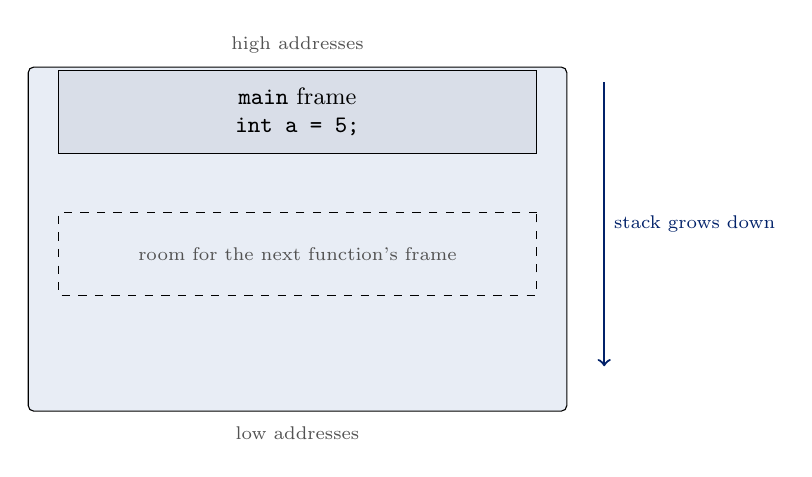
\begin{tikzpicture}[scale=0.95, every node/.style={scale=0.95}]
    % Diagram: one stack frame (main) with room below.
    % Coordinates: (x, y)
    %   outer region at (0,-1.5), width 7.2cm, height 4.6cm
    %   main frame at (0,0.2), width 6.4cm, height 1.1cm
    %   dashed "next frame" placeholder at (0,-1.7), width 6.4cm, height 1.1cm
    %   growth arrow x=4.1 from y=0.6 to y=-3.2
    \node[draw, fill=light-bg, minimum width=7.2cm, minimum height=4.6cm,
          rounded corners=2pt] at (0,-1.5) {};
    \node[font=\scriptsize, text=neutral] at (0,1.1) {high addresses};
    \node[draw, fill=primary-blue!15, minimum width=6.4cm, minimum height=1.1cm,
          align=center, font=\small] at (0,0.2)
          {\texttt{main} frame\\ \texttt{int a = 5;}};
    \node[draw, dashed, minimum width=6.4cm, minimum height=1.1cm,
          align=center, font=\scriptsize, text=neutral] at (0,-1.7)
          {room for the next function's frame};
    \draw[->, thick, color=primary-blue] (4.1,0.6) -- (4.1,-3.2)
      node[midway, right, font=\scriptsize] {stack grows down};
    \node[font=\scriptsize, text=neutral] at (0,-4.1) {low addresses};
  \end{tikzpicture}
  \end{center}
  \begin{itemize}
    \item Starting \texttt{main} creates one frame holding its local variables.
    \item Every new function call pushes a new frame just below the current one.
  \end{itemize}
\end{frame}

\begin{frame}{How the Stack Grows --- Step 2: \texttt{add} is called}
  \begin{center}
  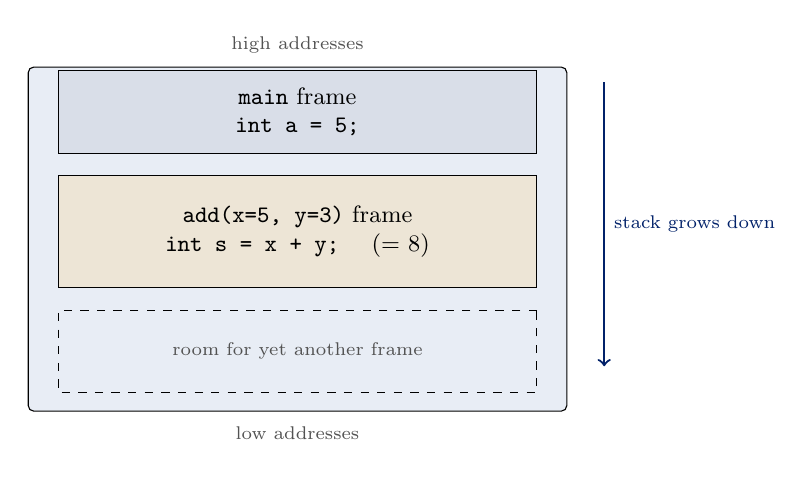
\begin{tikzpicture}[scale=0.95, every node/.style={scale=0.95}]
    % Diagram: main frame plus a second (add) frame pushed below.
    % Coordinates: (x, y)
    %   outer region at (0,-1.5), width 7.2cm, height 4.6cm
    %   main frame at (0,0.2), width 6.4cm, height 1.1cm
    %   add frame at (0,-1.4), width 6.4cm, height 1.5cm
    %   dashed "room" placeholder at (0,-3.0), width 6.4cm, height 1.1cm
    %   growth arrow x=4.1 from y=0.6 to y=-3.2
    \node[draw, fill=light-bg, minimum width=7.2cm, minimum height=4.6cm,
          rounded corners=2pt] at (0,-1.5) {};
    \node[font=\scriptsize, text=neutral] at (0,1.1) {high addresses};
    \node[draw, fill=primary-blue!15, minimum width=6.4cm, minimum height=1.1cm,
          align=center, font=\small] at (0,0.2)
          {\texttt{main} frame\\ \texttt{int a = 5;}};
    \node[draw, fill=primary-gold!25, minimum width=6.4cm, minimum height=1.5cm,
          align=center, font=\small] at (0,-1.4)
          {\texttt{add(x=5, y=3)} frame\\ \texttt{int s = x + y;} \quad (= 8)};
    \node[draw, dashed, minimum width=6.4cm, minimum height=1.1cm,
          align=center, font=\scriptsize, text=neutral] at (0,-3.0)
          {room for yet another frame};
    \draw[->, thick, color=primary-blue] (4.1,0.6) -- (4.1,-3.2)
      node[midway, right, font=\scriptsize] {stack grows down};
    \node[font=\scriptsize, text=neutral] at (0,-4.1) {low addresses};
  \end{tikzpicture}
  \end{center}
  \begin{itemize}
    \item The call to \texttt{add} pushed a second frame with its parameters and locals.
    \item The new frame sits at a \key{lower} address than \texttt{main}'s frame.
  \end{itemize}
\end{frame}

\begin{frame}{How the Stack Grows --- Step 3: \texttt{add} returns}
  \begin{center}
  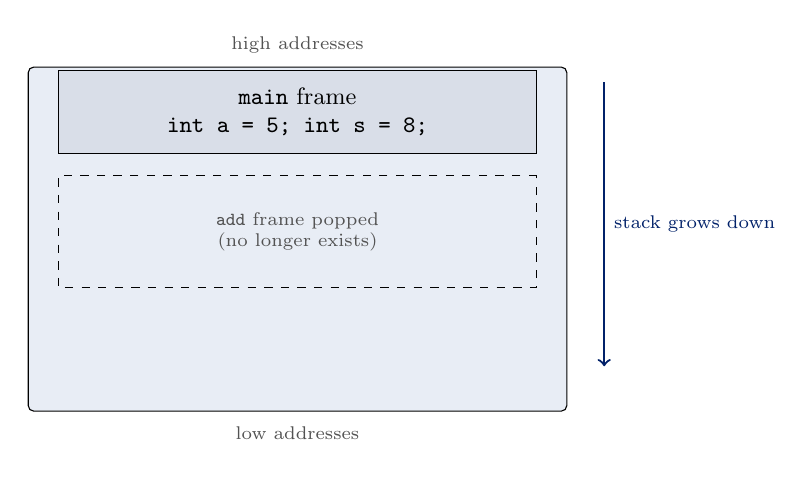
\begin{tikzpicture}[scale=0.95, every node/.style={scale=0.95}]
    % Diagram: main frame only; add frame shown as popped (dashed).
    % Coordinates: (x, y)
    %   outer region at (0,-1.5), width 7.2cm, height 4.6cm
    %   main frame at (0,0.2), width 6.4cm, height 1.1cm (now with s = 8)
    %   popped add frame at (0,-1.4), width 6.4cm, height 1.5cm (dashed)
    %   growth arrow x=4.1 from y=0.6 to y=-3.2
    \node[draw, fill=light-bg, minimum width=7.2cm, minimum height=4.6cm,
          rounded corners=2pt] at (0,-1.5) {};
    \node[font=\scriptsize, text=neutral] at (0,1.1) {high addresses};
    \node[draw, fill=primary-blue!15, minimum width=6.4cm, minimum height=1.1cm,
          align=center, font=\small] at (0,0.2)
          {\texttt{main} frame\\ \texttt{int a = 5; int s = 8;}};
    \node[draw, dashed, minimum width=6.4cm, minimum height=1.5cm,
          align=center, font=\scriptsize, text=neutral] at (0,-1.4)
          {\texttt{add} frame popped\\ (no longer exists)};
    \draw[->, thick, color=primary-blue] (4.1,0.6) -- (4.1,-3.2)
      node[midway, right, font=\scriptsize] {stack grows down};
    \node[font=\scriptsize, text=neutral] at (0,-4.1) {low addresses};
  \end{tikzpicture}
  \end{center}
  \begin{itemize}
    \item Returning popped the frame, and its memory is available again.
    \item The answer \texttt{8} was copied back into \texttt{main}'s frame.
  \end{itemize}
\end{frame}

\begin{frame}{The Stack: Automatic Storage}
  \begin{block}{Definition}
    A local variable is created when its function starts and destroyed when
    the function returns --- the program manages this automatically.
  \end{block}
  \begin{exampleblock}{Example}
    \texttt{int score = 80;} inside a function is a local variable: it is
    gone the moment that function returns.
  \end{exampleblock}
\end{frame}

\begin{frame}{Why Do We Need the Heap?}
  \begin{block}{A changing problem}
    The user enters the number of records only after the program starts.
  \end{block}
  \begin{itemize}
    \item We may need space for 3 records today and 300 tomorrow.
    \item We may want the records to remain after a helper function returns.
    \item A structure whose size is known only at run time cannot be given a
      fixed amount of storage at compile time
      \cite{Wirth2004_algorithms_data_structures}.
  \end{itemize}
  \key{The heap gives us memory whose size and lifetime we request at run time.}
  \muted{Wirth's argument, p.111: if the size is known only at run time, the
    storage must be allocated at run time too.}
\end{frame}

\begin{frame}{Check Your Prediction}
  \begin{block}{Which variable can outlive the function that created it?}
    \texttt{int score = 80;}\hfill or\hfill \texttt{int *p = malloc(sizeof(int));}
  \end{block}
  \begin{itemize}
    \item \texttt{score} belongs to its function call --- gone on return.
    \item The heap block remains until released with \texttt{free}.
  \end{itemize}
  \muted{The exact call for this --- \texttt{malloc} and \texttt{sizeof} ---
    is next.}
\end{frame}

\transitionslide{To use the heap, we need a handle on it --- a pointer.}

% =============================================================================
% ACT 3 --- POINTERS
% =============================================================================
\section{Pointers}

\sectiondivider{Section 3}{Pointers}

\begin{frame}{What Is a Pointer?}
  \begin{block}{Definition}
    A pointer is a variable that stores an address
    \cite{Wirth2004_algorithms_data_structures}.
  \end{block}
  \begin{itemize}
    \item An ordinary variable stores a value such as \texttt{80}.
    \item A pointer stores a place such as ``where the score lives''.
  \end{itemize}
  \begin{exampleblock}{One declaration}
    \texttt{int *p;} means: \texttt{p} can point to an \texttt{int}.
  \end{exampleblock}
\end{frame}

\begin{frame}{A Pointer Picture}
  \begin{center}
    % Diagram: pointer box pointing to value box. Coordinates: (x,y)
    %   p box at (-2.5,0), w=3.0 h=1.0
    %   value box at (2.5,0), w=3.0 h=1.0
    %   arrow p.east -> x.west (horizontal, y=0, clear)
    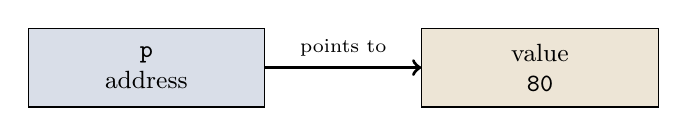
\begin{tikzpicture}[every node/.style={font=\small}]
      \node[draw, fill=primary-blue!15, minimum width=3.0cm, minimum height=1cm,
        align=center]
        (p) at (-2.5,0) {\texttt{p}\\address};
      \node[draw, fill=primary-gold!25, minimum width=3.0cm, minimum height=1cm,
        align=center]
        (x) at (2.5,0) {value\\\texttt{80}};
      \draw[->, very thick] (p.east) -- (x.west)
        node[midway, above, font=\scriptsize] {points to};
    \end{tikzpicture}
  \end{center}
  \begin{itemize}
    \item \texttt{p} does not contain the score itself.
    \item \texttt{p} tells us where the score can be found.
  \end{itemize}
\end{frame}

\begin{frame}[fragile]{A Pointer Can Reach a Node}
  \begin{block}{A two-field node}
\begin{semiverbatim}
struct node \{
  int data;
  struct node *next;
\};
\end{semiverbatim}
  \end{block}
  \begin{itemize}
    \item \texttt{data} stores the value.
    \item \texttt{next} stores the address of another node, or \texttt{NULL}.
  \end{itemize}
  \muted{This is the building block for a linked list in a later week. (The
    list handle will be called \texttt{head}; here the node is just
    \texttt{p}.)}
\end{frame}

\begin{frame}{The Safe Empty Pointer}
  \begin{block}{Definition}
    \texttt{NULL} means a pointer is not pointing to a valid object.
  \end{block}
  \begin{exampleblock}{Example}
    \texttt{struct node *p = NULL;} means ``this pointer reaches nothing yet''.
  \end{exampleblock}
  \begin{itemize}
    \item Check a pointer against \texttt{NULL} before using what it points to.
    \item Never read through an empty pointer.
  \end{itemize}
\end{frame}

\transitionslide{Now let us actually request a block of heap memory and use it.}

% =============================================================================
% ACT 4 --- ONE HEAP BLOCK
% =============================================================================
\section{One Heap Block}

\sectiondivider{Section 4}{One Heap Block}

\begin{frame}[fragile]{Requesting Memory: \texttt{malloc}}
  \begin{block}{Definition}
    \texttt{malloc(n)} asks the heap for \texttt{n} bytes and returns their
    address, or \texttt{NULL} if the request fails.
  \end{block}
\begin{semiverbatim}
int *p = malloc(sizeof(int));
if (p == NULL) return 1;
*p = 80;
\end{semiverbatim}
  \muted{Always check the result against \texttt{NULL} before using it.}
\end{frame}

\begin{frame}[fragile]{\texttt{sizeof}: the Unit of Every Request}
  \begin{block}{Definition}
    \texttt{sizeof(T)} is the compile-time size, in bytes, of type \texttt{T}.
  \end{block}
\begin{semiverbatim}
sizeof(int)          \textcolor{neutral}{// typically 4}
sizeof(struct node)  \textcolor{neutral}{// data field + next field}
\end{semiverbatim}
  \begin{itemize}
    \item \texttt{malloc} never knows how big an \texttt{int} is on its own.
    \item \texttt{sizeof} is what tells it --- every allocation request uses it.
  \end{itemize}
\end{frame}

\begin{frame}[fragile]{Zero-Initialized Memory: \texttt{calloc}}
  \begin{block}{Definition}
    \texttt{calloc(n, size)} allocates space for \texttt{n} items of
    \texttt{size} bytes each, and sets every byte to \texttt{0}.
  \end{block}
\begin{semiverbatim}
int *counts = calloc(5, sizeof(int));
if (counts == NULL) return 1;
\end{semiverbatim}
  \key{calloc} zero-initializes; \key{malloc} does not.
\end{frame}

\begin{frame}{Worked Example: \texttt{malloc} vs.\ \texttt{calloc}}
  \begin{center}
    % Diagram: two 4-byte blocks side by side, malloc (garbage) vs calloc (zeros).
    % Coordinates: (x,y) -- no lines, no bends; two independent boxes.
    %   malloc box at (-2.4, 0), w=3.8cm h=1.1cm
    %   calloc box at (2.4, 0), w=3.8cm h=1.1cm
    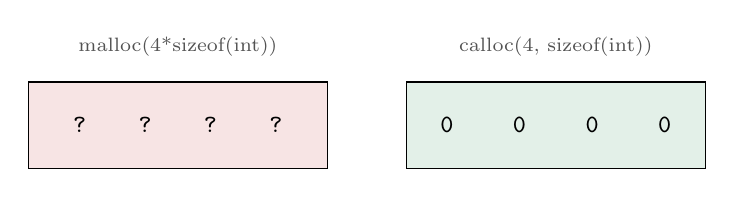
\begin{tikzpicture}[every node/.style={font=\small}]
      % Diagram: two independent 4-byte blocks, no connecting lines.
      % Coordinates: (x,y)
      %   malloc label at (-2.4, 1.0); malloc box at (-2.4, 0), w=3.8cm h=1.1cm
      %     (box top edge at y=0.55; label at y=1.0 clears it by 0.45cm >= 0.4cm)
      %   calloc label at (2.4, 1.0); calloc box at (2.4, 0), w=3.8cm h=1.1cm
      \node[font=\scriptsize, text=neutral] at (-2.4,1.0) {malloc(4*sizeof(int))};
      \node[draw, fill=negative!12, minimum width=3.8cm, minimum height=1.1cm,
        align=center, font=\ttfamily\small]
        (m) at (-2.4,0) {? \quad ? \quad ? \quad ?};
      \node[font=\scriptsize, text=neutral] at (2.4,1.0) {calloc(4, sizeof(int))};
      \node[draw, fill=positive!12, minimum width=3.8cm, minimum height=1.1cm,
        align=center, font=\ttfamily\small]
        (c) at (2.4,0) {0 \quad\; 0 \quad\; 0 \quad\; 0};
    \end{tikzpicture}
  \end{center}
  \begin{itemize}
    \item \texttt{malloc} hands back four \key{unspecified} bytes --- reading
      them before writing is undefined behaviour.
    \item \texttt{calloc} hands back four bytes already \key{set to zero}.
  \end{itemize}
\end{frame}

\begin{frame}[fragile]{Resizing a Block: \texttt{realloc}}
  \begin{block}{Definition}
    \texttt{realloc(p, newsize)} resizes the block \texttt{p} points to,
    preserving its existing content up to the smaller of the old and new
    sizes. The block \key{may move} --- always keep the returned pointer.
  \end{block}
\begin{semiverbatim}
int *bigger = realloc(p, 10 * sizeof(int));
if (bigger == NULL) return 1;  \textcolor{neutral}{// p is still valid here}
p = bigger;
\end{semiverbatim}
\end{frame}

\begin{frame}{Worked Example: Growing an Array with \texttt{realloc}}
  \begin{block}{Trace}
    Start with \texttt{p = malloc(3 * sizeof(int))} holding \texttt{10 20 30}.
  \end{block}
  \begin{enumerate}
    \item \texttt{p = realloc(p, 5 * sizeof(int));}
    \item The first three ints (\texttt{10 20 30}) are copied to the new block.
    \item The two new slots are \key{unspecified} --- \texttt{realloc} does
      not zero new space, only \texttt{calloc} zeros space.
  \end{enumerate}
  \muted{If \texttt{realloc} returns \texttt{NULL}, the original block at
    \texttt{p} is untouched and still valid --- never overwrite \texttt{p}
    with the raw result before checking it.}
\end{frame}

\begin{frame}[fragile]{Allocate a Complete Node}
  \begin{block}{A safer engineering pattern}
\begin{semiverbatim}
struct node *p = malloc(sizeof(struct node));
if (p == NULL) return 1;
p->data = 42;
p->next = NULL;
\end{semiverbatim}
  \end{block}
  \begin{itemize}
    \item \texttt{sizeof(struct node)} asks for exactly one node's bytes.
    \item \texttt{p->data} means: the \texttt{data} field of the node \texttt{p}
      points at.
    \item This node has a clear end: \texttt{p->next == NULL}.
  \end{itemize}
\end{frame}

\begin{frame}{Audit the Node Before You Ship It}
  \begin{block}{Review checklist}
    A small program is not finished when it compiles.
  \end{block}
  \begin{enumerate}
    \item Was the allocation checked against \texttt{NULL}?
    \item Was every field initialised before the node was used?
    \item Is there exactly one clear owner responsible for \texttt{free(p)}?
    \item Can the program reach the node later, or has its pointer been lost?
  \end{enumerate}
\end{frame}

\begin{frame}{Trace It Before Running It}
  \begin{block}{After these lines, what is true?}
    \texttt{int *p = malloc(sizeof(int)); *p = 80;}
  \end{block}
  \begin{enumerate}
    \item \texttt{p} contains an address.
    \item The heap block at that address contains \texttt{80}.
    \item The name \texttt{p} itself is not the heap block.
  \end{enumerate}
  \begin{exampleblock}{Challenge}
    Which line would fail if \texttt{p == NULL}?
  \end{exampleblock}
\end{frame}

\begin{frame}{What Happened?}
  \begin{center}
    % Diagram: stack pointer box pointing to heap value box. Coordinates: (x,y)
    %   p box at (-2.5,0), w=3cm h=1cm
    %   heap box at (2.5,0), w=3cm h=1cm
    %   arrow p.east -> box.west
    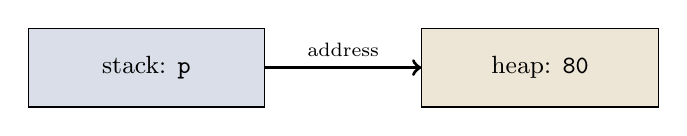
\begin{tikzpicture}[every node/.style={font=\small}]
      \node[draw, fill=primary-blue!15, minimum width=3cm, minimum height=1cm]
        (p) at (-2.5,0) {stack: \texttt{p}};
      \node[draw, fill=primary-gold!25, minimum width=3cm, minimum height=1cm]
        (box) at (2.5,0) {heap: \texttt{80}};
      \draw[->, very thick] (p.east) -- (box.west)
        node[midway, above, font=\scriptsize] {address};
    \end{tikzpicture}
  \end{center}
  \begin{enumerate}
    \item C found a free heap block.
    \item The address was stored in \texttt{p}.
    \item We used \texttt{*p} to write the value \texttt{80} there.
  \end{enumerate}
\end{frame}

\begin{frame}{How the Heap Grows --- Step 1: a block of three ints}
  \begin{center}
  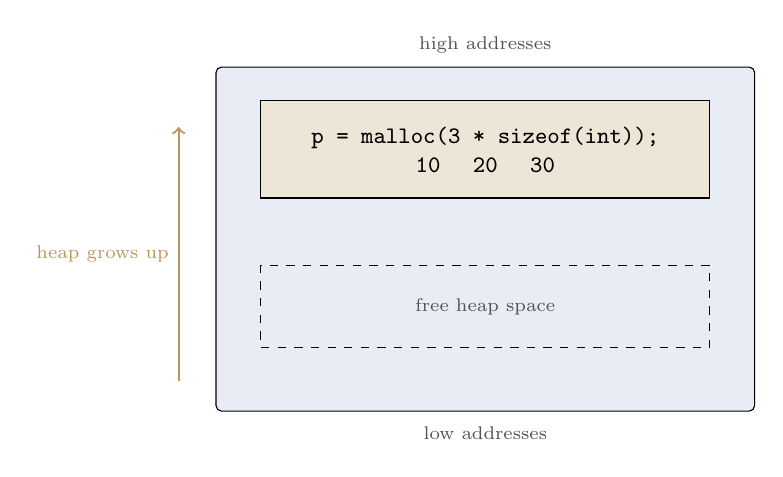
\begin{tikzpicture}[scale=0.95, every node/.style={scale=0.95}]
    % Diagram: one heap block (p) with free space below.
    % Coordinates: (x, y)
    %   outer region at (0,-1.5), width 7.2cm, height 4.6cm
    %   p block at (0,-0.3), width 6.0cm, height 1.3cm
    %   dashed "free heap space" at (0,-2.4), width 6.0cm, height 1.1cm
    %   growth arrow x=-4.1 from y=-3.4 to y=0.0
    \node[draw, fill=light-bg, minimum width=7.2cm, minimum height=4.6cm,
          rounded corners=2pt] at (0,-1.5) {};
    \node[font=\scriptsize, text=neutral] at (0,1.1) {high addresses};
    \node[draw, fill=primary-gold!25, minimum width=6.0cm, minimum height=1.3cm,
          align=center, font=\small] at (0,-0.3)
          {\texttt{p = malloc(3 * sizeof(int));}\\ \texttt{10} \quad \texttt{20} \quad \texttt{30}};
    \node[draw, dashed, minimum width=6.0cm, minimum height=1.1cm,
          align=center, font=\scriptsize, text=neutral] at (0,-2.4)
          {free heap space};
    \draw[->, thick, color=primary-gold] (-4.1,-3.4) -- (-4.1,0.0)
      node[midway, left, font=\scriptsize] {heap grows up};
    \node[font=\scriptsize, text=neutral] at (0,-4.1) {low addresses};
  \end{tikzpicture}
  \end{center}
  \begin{itemize}
    \item One \texttt{malloc} with room for three integers \key{grew the used heap} upward.
    \item The block survives after the allocating function returns.
  \end{itemize}
\end{frame}

\begin{frame}{How the Heap Grows --- Step 2: a second block}
  \begin{center}
  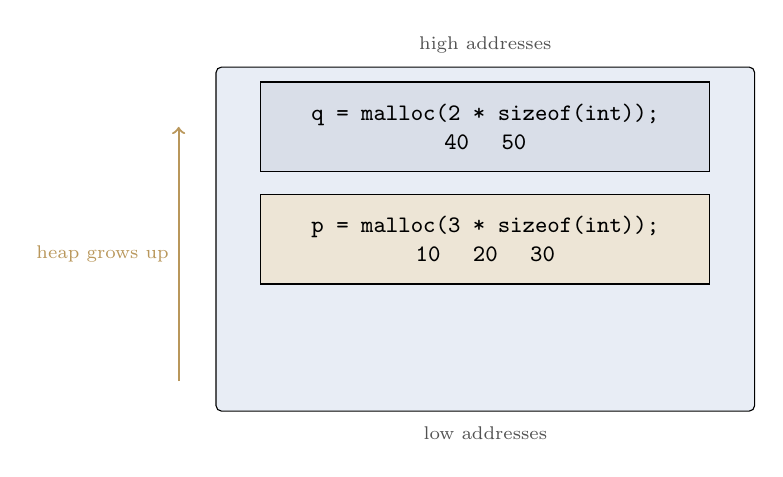
\begin{tikzpicture}[scale=0.95, every node/.style={scale=0.95}]
    % Diagram: two heap blocks, q above p.
    % Coordinates: (x, y)
    %   outer region at (0,-1.5), width 7.2cm, height 4.6cm
    %   q block at (0,0.0), width 6.0cm, height 1.2cm
    %   p block at (0,-1.5), width 6.0cm, height 1.2cm
    %   growth arrow x=-4.1 from y=-3.4 to y=0.0
    \node[draw, fill=light-bg, minimum width=7.2cm, minimum height=4.6cm,
          rounded corners=2pt] at (0,-1.5) {};
    \node[font=\scriptsize, text=neutral] at (0,1.1) {high addresses};
    \node[draw, fill=primary-gold!25, minimum width=6.0cm, minimum height=1.2cm,
          align=center, font=\small] at (0,-1.5)
          {\texttt{p = malloc(3 * sizeof(int));}\\ \texttt{10} \quad \texttt{20} \quad \texttt{30}};
    \node[draw, fill=primary-blue!15, minimum width=6.0cm, minimum height=1.2cm,
          align=center, font=\small] at (0,0.0)
          {\texttt{q = malloc(2 * sizeof(int));}\\ \texttt{40} \quad \texttt{50}};
    \draw[->, thick, color=primary-gold] (-4.1,-3.4) -- (-4.1,0.0)
      node[midway, left, font=\scriptsize] {heap grows up};
    \node[font=\scriptsize, text=neutral] at (0,-4.1) {low addresses};
  \end{tikzpicture}
  \end{center}
  \begin{itemize}
    \item The second request placed \texttt{q}'s block at a \key{higher} address.
    \item Blocks are independent; each keeps its own data.
  \end{itemize}
\end{frame}

\begin{frame}{How the Heap Grows --- Step 3: \texttt{free} returns a block}
  \begin{center}
  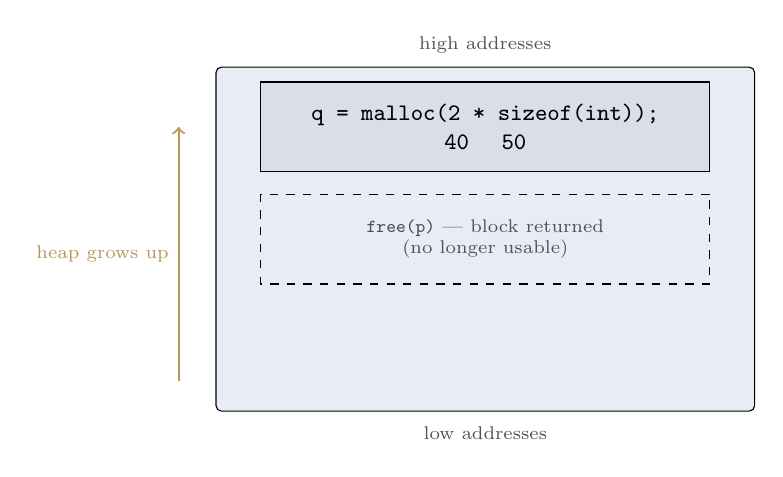
\begin{tikzpicture}[scale=0.95, every node/.style={scale=0.95}]
    % Diagram: q block remains; p block shown freed (dashed).
    % Coordinates: (x, y)
    %   outer region at (0,-1.5), width 7.2cm, height 4.6cm
    %   q block at (0,0.0), width 6.0cm, height 1.2cm
    %   freed p block at (0,-1.5), width 6.0cm, height 1.2cm (dashed)
    %   growth arrow x=-4.1 from y=-3.4 to y=0.0
    \node[draw, fill=light-bg, minimum width=7.2cm, minimum height=4.6cm,
          rounded corners=2pt] at (0,-1.5) {};
    \node[font=\scriptsize, text=neutral] at (0,1.1) {high addresses};
    \node[draw, dashed, minimum width=6.0cm, minimum height=1.2cm,
          align=center, font=\scriptsize, text=neutral] at (0,-1.5)
          {\texttt{free(p)} --- block returned\\ (no longer usable)};
    \node[draw, fill=primary-blue!15, minimum width=6.0cm, minimum height=1.2cm,
          align=center, font=\small] at (0,0.0)
          {\texttt{q = malloc(2 * sizeof(int));}\\ \texttt{40} \quad \texttt{50}};
    \draw[->, thick, color=primary-gold] (-4.1,-3.4) -- (-4.1,0.0)
      node[midway, left, font=\scriptsize] {heap grows up};
    \node[font=\scriptsize, text=neutral] at (0,-4.1) {low addresses};
  \end{tikzpicture}
  \end{center}
  \begin{itemize}
    \item \texttt{free(p)} gives \texttt{p}'s block back to the system.
    \item \texttt{q}'s block is untouched, and the used heap can shrink again.
  \end{itemize}
\end{frame}

\begin{frame}[fragile]{Returning the Memory: \texttt{free}}
  \begin{block}{Definition}
    \texttt{free(p)} returns the heap block \texttt{p} points to back to the
    system. Every \texttt{malloc}/\texttt{calloc}/\texttt{realloc} needs a
    matching \texttt{free}.
  \end{block}
\begin{semiverbatim}
free(p);
p = NULL;
\end{semiverbatim}
  \good{Request memory, use it, return it.}
\end{frame}

\begin{frame}{Two Beginner Mistakes}
  \begin{itemize}
    \item \bad{Memory leak}: forget to call \texttt{free}; the block stays
      reserved forever.
    \item \bad{Dangling pointer}: use a pointer after its block was freed.
  \end{itemize}
  \begin{exampleblock}{Simple habit}
    Keep track of who requested the memory and who will return it.
  \end{exampleblock}
\end{frame}

\transitionslide{Memory and pointers are the machinery. The contract is the map.}

% =============================================================================
% ACT 5 --- SIMPLE CONTRACTS
% =============================================================================
\section{Simple Contracts}

\sectiondivider{Section 5}{Simple Contracts}

\begin{frame}{What Is an ADT?}
  \begin{block}{Definition}
    An ADT describes \emph{what} we can do with data, without saying
    \emph{how} it is stored --- ``a set of values and a set of operations on
    those values'' (Sedgewick, p.64)
    \cite{Sedgewick2011_algorithms}.
  \end{block}
  \muted{Karumanchi (p.18, PDF) frames the same idea as a declaration of data
    plus a declaration of operations
    \cite{Karumanchi2017_data_structures_algorithms_made_easy}.}
\end{frame}

\begin{frame}{Worked Example: A Very Small Bag}
  \begin{block}{The contract}
    A bag of integers supports three operations:
  \end{block}
  \begin{enumerate}
    \item \texttt{insert(x)} --- put \texttt{x} into the bag.
    \item \texttt{member(x)} --- answer whether \texttt{x} is present.
    \item \texttt{size()} --- report how many items are present.
  \end{enumerate}
  \muted{The contract does not yet say whether the bag uses an array or a
    list. A bag is one of Sedgewick's three collection types (p.120)
    \cite{Sedgewick2011_algorithms}.}
\end{frame}

\begin{frame}{This Course Is a Tour of ADTs}
  \begin{block}{The pattern you will see every week}
    Linked Lists, Stacks, Queues, Priority Queues, Binary Trees, Hash Tables,
    and Graphs are all commonly used ADTs
    \cite{Karumanchi2017_data_structures_algorithms_made_easy}.
  \end{block}
  \muted{Watch for this shape every week: ``What is a Stack?'' then
    ``Stack ADT'' then ``Implementation.''}
\end{frame}

\begin{frame}{One Contract, Two Possible Implementations}
  \begin{center}
    % Diagram: contract box on top, two implementation boxes below.
    % Coordinates: (x,y)
    %   contract (0,2), w=5cm h=1cm
    %   array (-2.5,0), w=3.5cm h=0.9cm
    %   list (2.5,0), w=3.5cm h=0.9cm
    %   arrows contract -> array / contract -> list (vertical/angled, clear)
    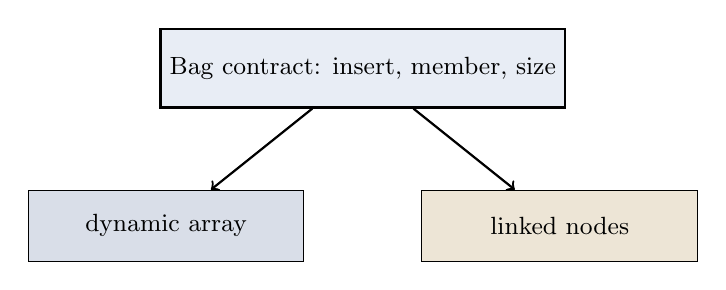
\begin{tikzpicture}[every node/.style={font=\small}]
      \node[draw, thick, fill=light-bg, minimum width=5cm, minimum height=1cm]
        (adt) at (0,2) {Bag contract: insert, member, size};
      \node[draw, fill=primary-blue!15, minimum width=3.5cm, minimum height=0.9cm]
        (array) at (-2.5,0) {dynamic array};
      \node[draw, fill=primary-gold!25, minimum width=3.5cm, minimum height=0.9cm]
        (list) at (2.5,0) {linked nodes};
      \draw[->, thick] (adt) -- (array);
      \draw[->, thick] (adt) -- (list);
    \end{tikzpicture}
  \end{center}
  \begin{itemize}
    \item Same operations, different internal arrangement.
    \item The caller's code does not change when the bottom box does.
  \end{itemize}
\end{frame}

\begin{frame}{Contract or Implementation?}
  \begin{block}{Classify each statement}
    Is it part of the contract, or part of one implementation?
  \end{block}
  \begin{enumerate}
    \item ``\texttt{member(7)} answers yes or no.''
    \item ``The values are stored in an array.''
    \item ``\texttt{size()} reports the number of values.''
  \end{enumerate}
  \muted{The first and third describe what users can ask (contract). The
    second describes how (implementation).}
\end{frame}

\begin{frame}{Week 1 Summary}
  \begin{itemize}
    \item \key{Structure:} sequence, selection, iteration build every program.
    \item \key{Memory:} the stack holds short-lived locals; the heap holds
      memory requested while the program runs.
    \item \key{Pointers:} a pointer stores an address; \texttt{NULL} means
      ``points to nothing.''
    \item \key{Dynamic memory:} \texttt{malloc}/\texttt{calloc}/\texttt{realloc}
      request, \texttt{free} returns.
    \item \key{ADTs:} state operations first (a contract); a data structure
      is the implementation that honours it.
  \end{itemize}
  \begin{exampleblock}{Next week}
    We learn how to talk about the amount of work an operation needs ---
    $T(n)$, $O$/$\Omega$/$\Theta$, and best/worst/average case.
  \end{exampleblock}
\end{frame}

\begin{frame}[allowframebreaks]{References}
  \footnotesize
  \bibliographystyle{plain}
  \bibliography{../../Bibliography_base}
\end{frame}

\end{document}
